\chapter{Implementation} \label{implementation}

\section{Authentication Policy}
With regard to the design of the authentication policies, conditional flows are used to fulfill the requirements for authentication policies.
The main difference is the additional lifecycle management provided for them with particular validations.
Reusing existing components is beneficial in this case as the implementation is simplified without introducing any other similar components.

In order to differentiate authentication flow and authentication policy, the parent authentication flow \textit{Authentication policies - PARENT} is provided to contain only authentication policies.
Moreover, every policy has the prefix \textit{"POLICY - "} for its alias to mark it as the authentication policy.
The validation and management for authentication policies are done through the specific \textit{Data Access Object} (DAO), shown in Section \ref{impl-authn-policies-dao}. 

As the authentication policies need to be managed from the outside world, the \textit{REST API} has been introduced with a detailed description in Section \ref{impl-authn-policies-rest}.
The administrator console, as a client application, also uses the Keycloak REST API to manage all entities.

\begin{figure}[htbp]
  \centering
  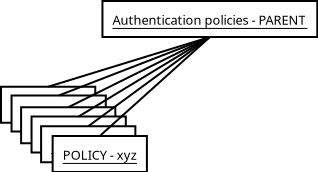
\includegraphics[width=0.5\textwidth]{img/sections/6-implementation/auth-policies-parent.png}
  \caption{Authentication Policies Parent.}
  \label{fig:impl-authn-policies-parent}
\end{figure}

\newpage

\subsection{Data Access Object} \label{impl-authn-policies-dao}
Data Access Object (DAO) pattern in software engineering abstracts database operations, shielding application logic from database sophistication and adhering to the single responsibility principle.\cite{impl-dao}

It is used to manage authentication policies as part of the separation from the authentication flows.
It provides necessary validation above the database layer and provides the functionality to properly mark conditional flow as an authentication policy.

The signature of operations for the authentication policy DAO is declared via the \textit{AuthnPolicyProvider} as shown in Figure \ref{fig:impl-authn-policies-provider-diagram}.

\begin{figure}[htbp]
  \centering
  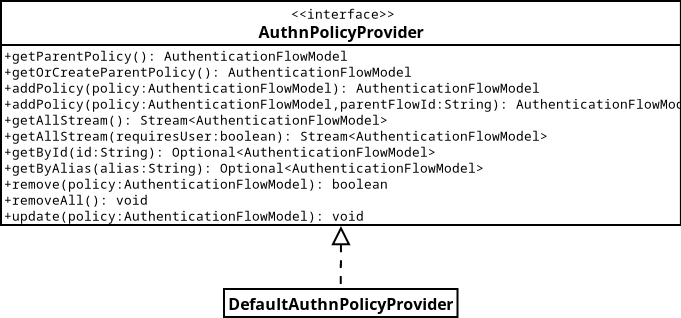
\includegraphics[width=1\textwidth]{img/sections/6-implementation/authn-policy-provider-diagram.png}
  \caption{Authentication Policy Provider.}
  \label{fig:impl-authn-policies-provider-diagram}
\end{figure}

\newpage

The interface \textit{AuthnPolicyProvider} consists of the basic CRUD operations that can be made on authentication policies, such as:

\begin{itemize}
    \item \textit{getParentPolicy()} -- retrieve the parent \textit{Authentication policies - PARENT} flow.
    \item \textit{getOrCreateParentPolicy()} -- retrieve, or create if it does not exist, the parent \textit{Authentication policies - PARENT} flow.
    \item \textit{addPolicy(policy)} -- add a new policy \textit{policy} with the default parent flow.
    \item \textit{addPolicy(policy, parentFlowId)} -- add a new policy \textit{policy} with the parent flow \textit{parentFlowId}.
    \item \textit{getAllStream()} -- retrieve a stream of all authentication policies.
    \item \textit{getAllStream(requiresUser)} -- retrieve a stream of all authentication policies with the execution phase equal to \textit{requiresUser} attribute.
    \item \textit{getById(id)} -- retrieve an authentication policy found by provided ID via the \textit{id} attribute.
    \item \textit{getByAlias(alias)} -- retrieve an authentication policy found by provided alias via the \textit{alias} attribute.
    \item \textit{remove(policy)} -- remove a policy defined in the \textit{policy} attribute.
    \item \textit{removeAll()} -- remove all authentication policies.
    \item \textit{update(policy)} -- update an authentication policy provided via the \textit{policy} attribute.
\end{itemize}

\newpage

\subsubsection{Add Authentication Policy}
One of the most interesting examples of implementing methods of the \textit{AuthnPolicyProvider} interface is the \textit{addPolicy()} method shown in Figure \ref{fig:impl-authn-policies-add-policy-diagram}.
That method is responsible for creating a new authentication policy based on the parameters.

\begin{figure}[htbp]
  \centering
  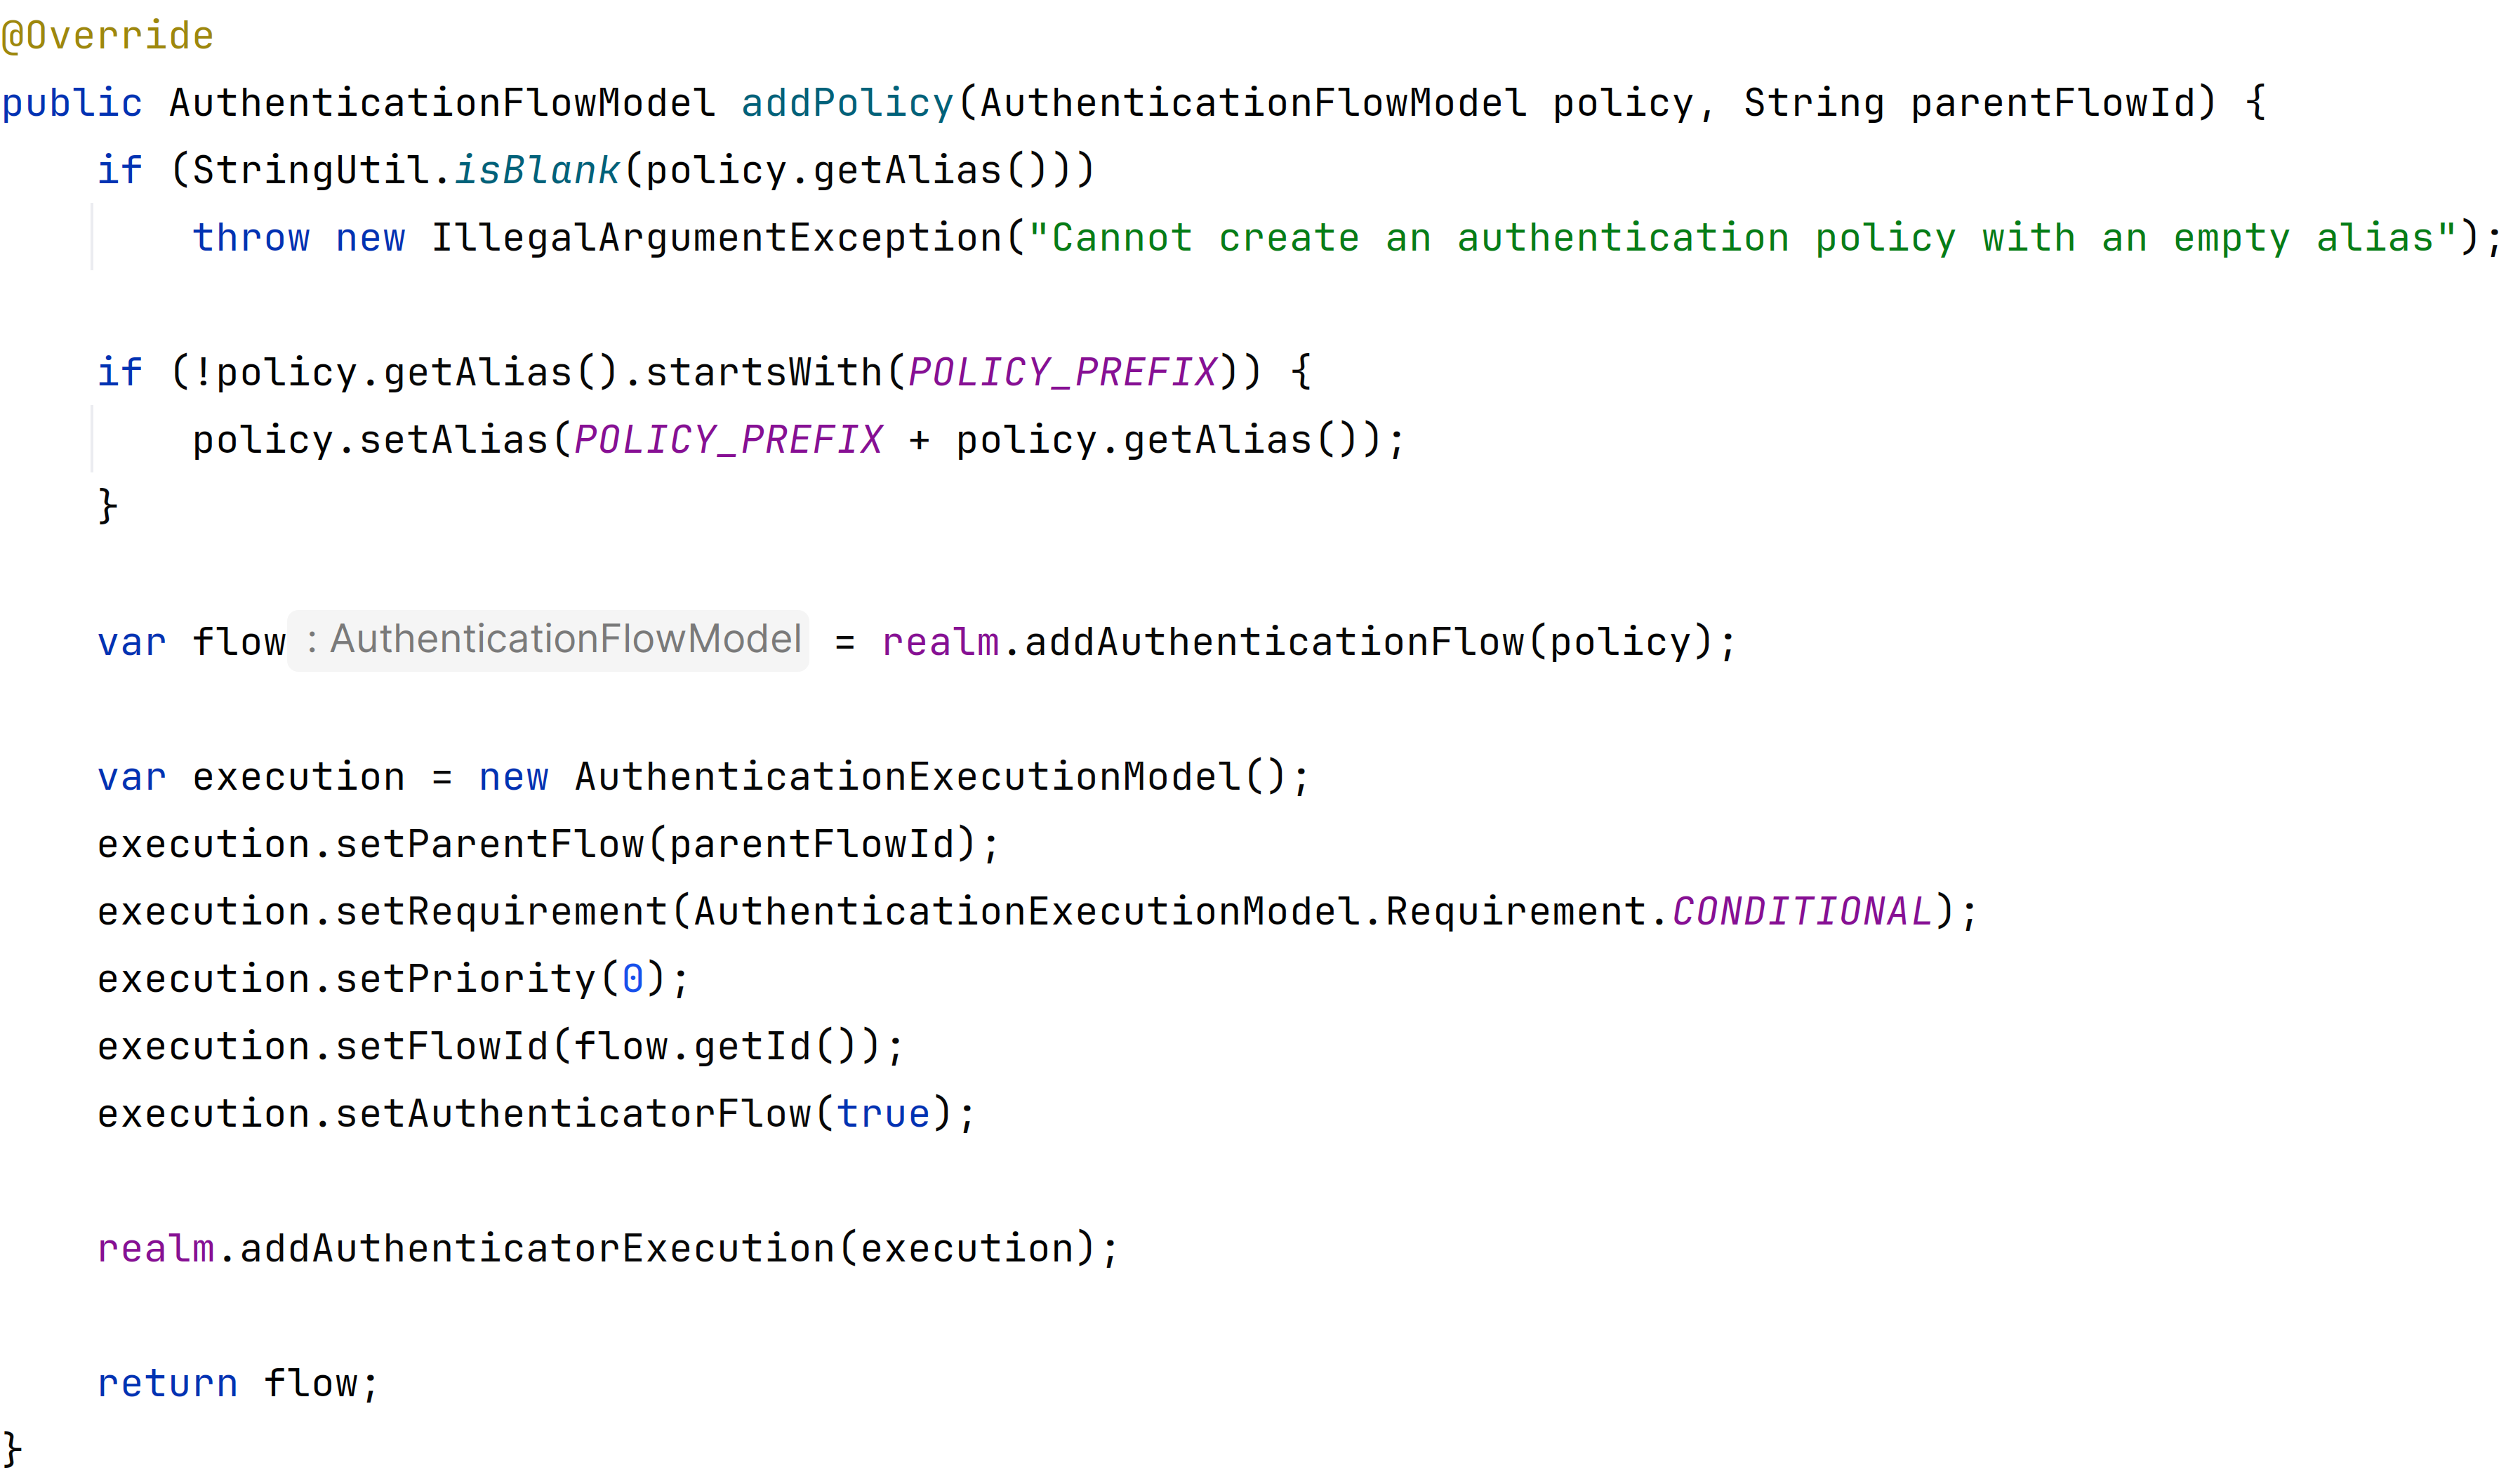
\includegraphics[width=1.05\textwidth]{img/sections/6-implementation/authnPolicyAddPolicy.png}
  \caption{Add Policy Method.}
  \label{fig:impl-authn-policies-add-policy-diagram}
\end{figure}

First of all, the alias must not be empty.
Otherwise, the exception is thrown.
If the alias does not start with the prefix \textit{"POLICY - "}, it is automatically added to the alias.
The last part of the execution is to create a conditional flow where the parent flow is the common parent authentication flow for all authentication policies.
The newly created authentication policy is returned.

\newpage

\subsubsection{Retrieve Authentication Policies}

Another method worth mentioning is the \textit{getAllStream(requiresUser)}, shown in Figure \ref{fig:impl-authn-policies-get-all}.
The method returns all authentication policies that match the \textit{requiresUser} Boolean attribute.
Specifically, it iterates over all policies, and if there is some requirement to require a user, it automatically includes it in the final stream.
It does not consider several layers of authentication policies hierarchy.
If the execution authenticator implements the \textit{ConfigurableRequirements} interface, the condition of whether it requires a user is evaluated dynamically.

\begin{figure}[htbp]
  \centering
  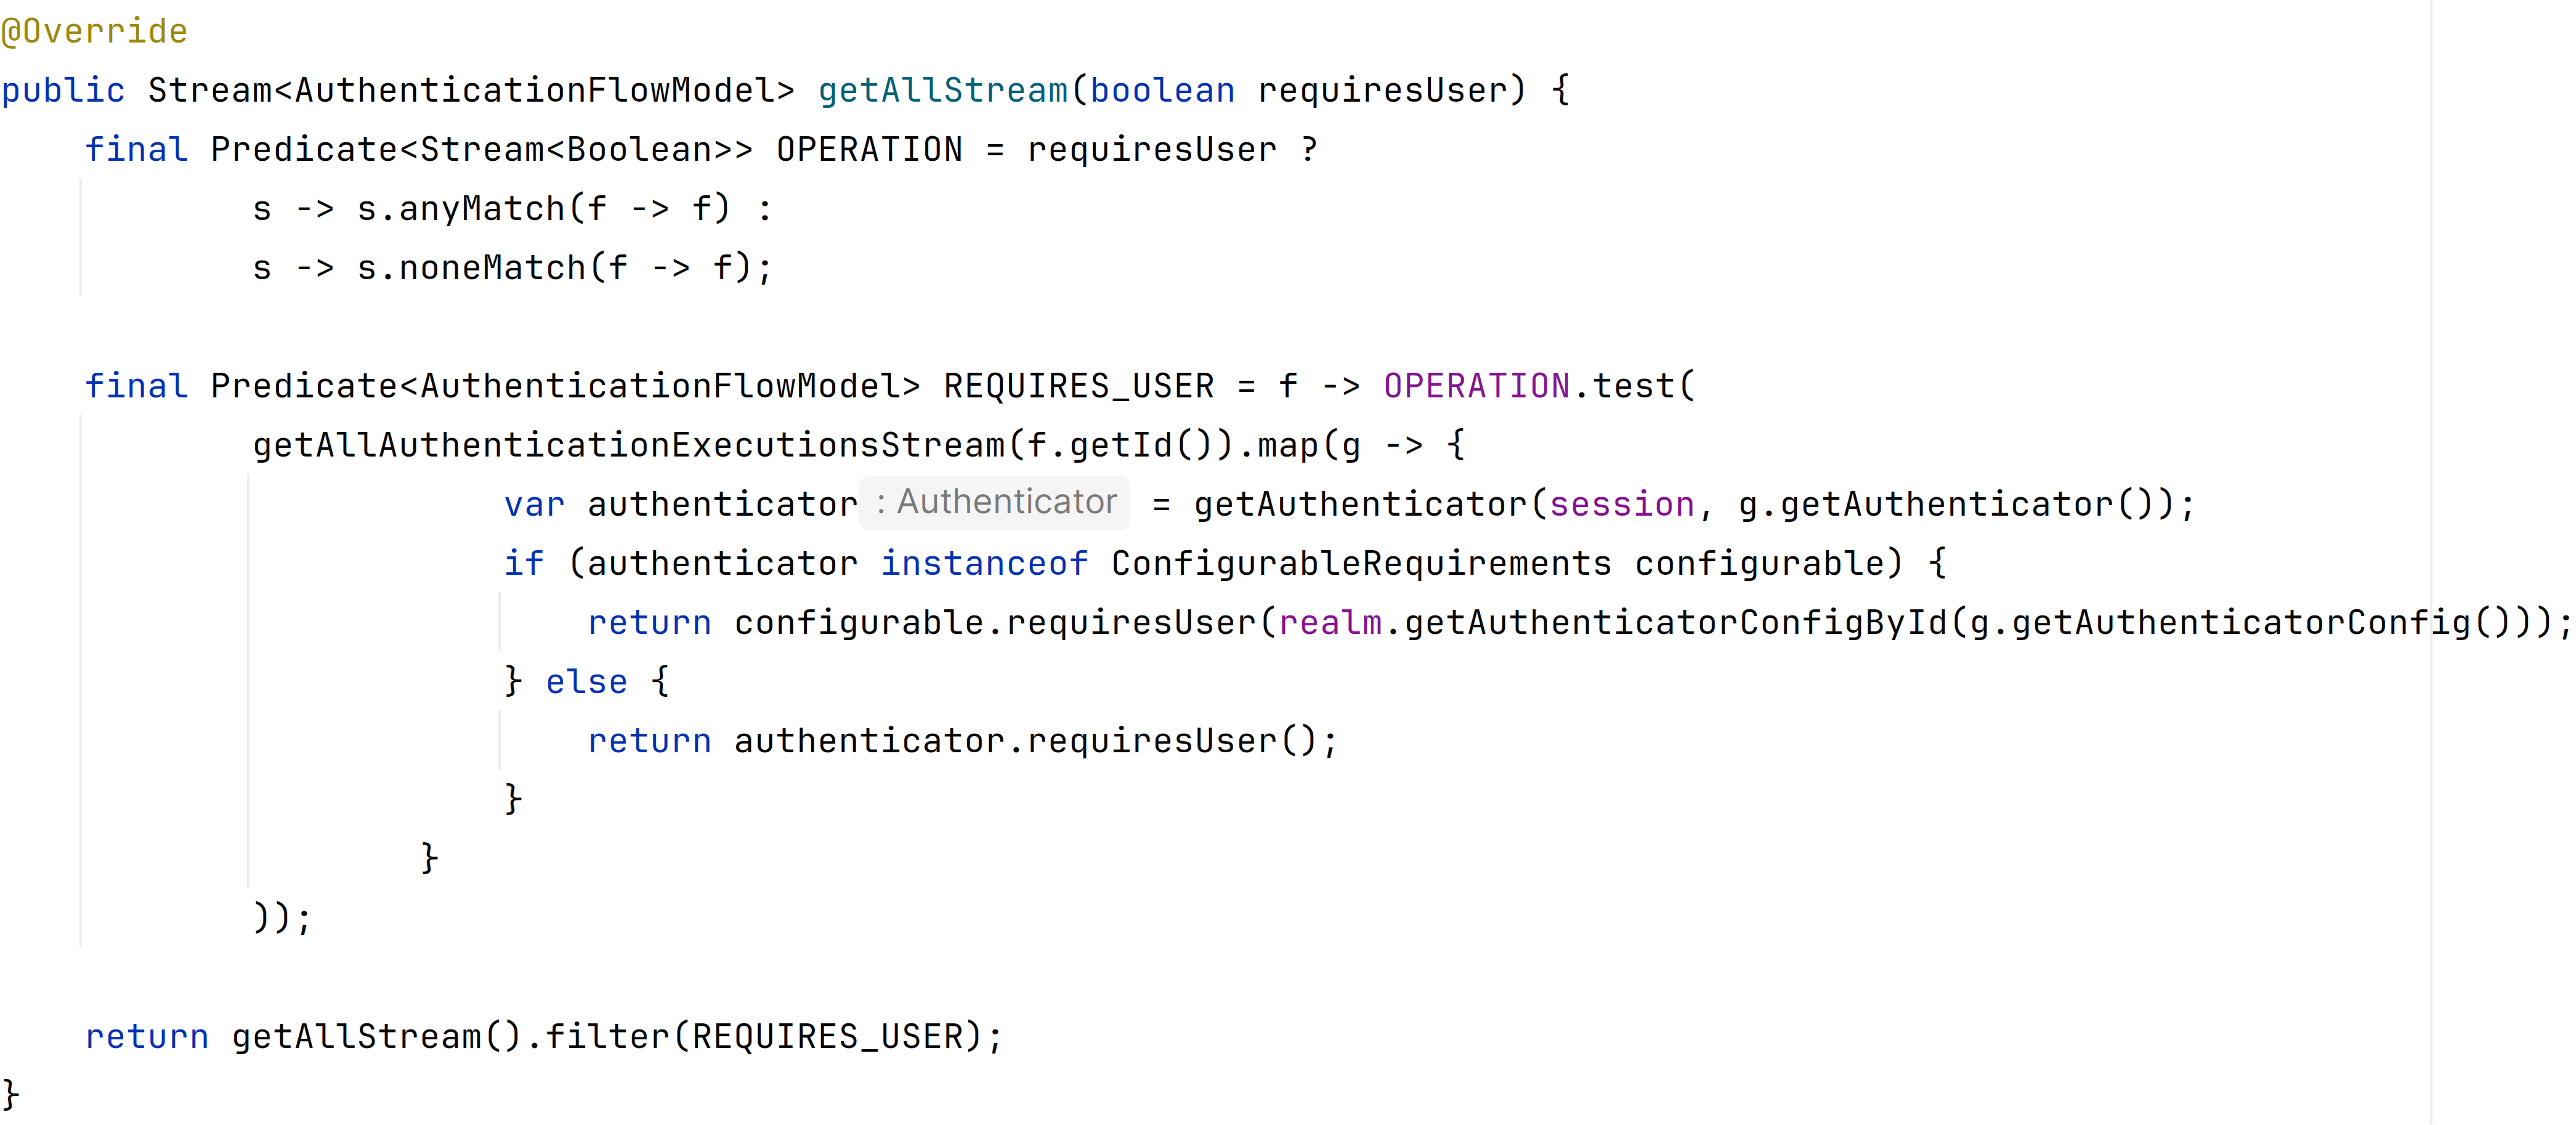
\includegraphics[width=1\textwidth]{img/sections/6-implementation/authnPolicyGetAllStream.png}
  \caption{Get All Authentication Policies.}
  \label{fig:impl-authn-policies-get-all}
\end{figure}

The helper method \textit{getAllAuthenticationExecutionsStream} shown in Figure \ref{fig:impl-authn-policies-get-all-execs} returns all executions included in the authentication policy with the usage of recursion.

\begin{figure}[htbp]
  \centering
  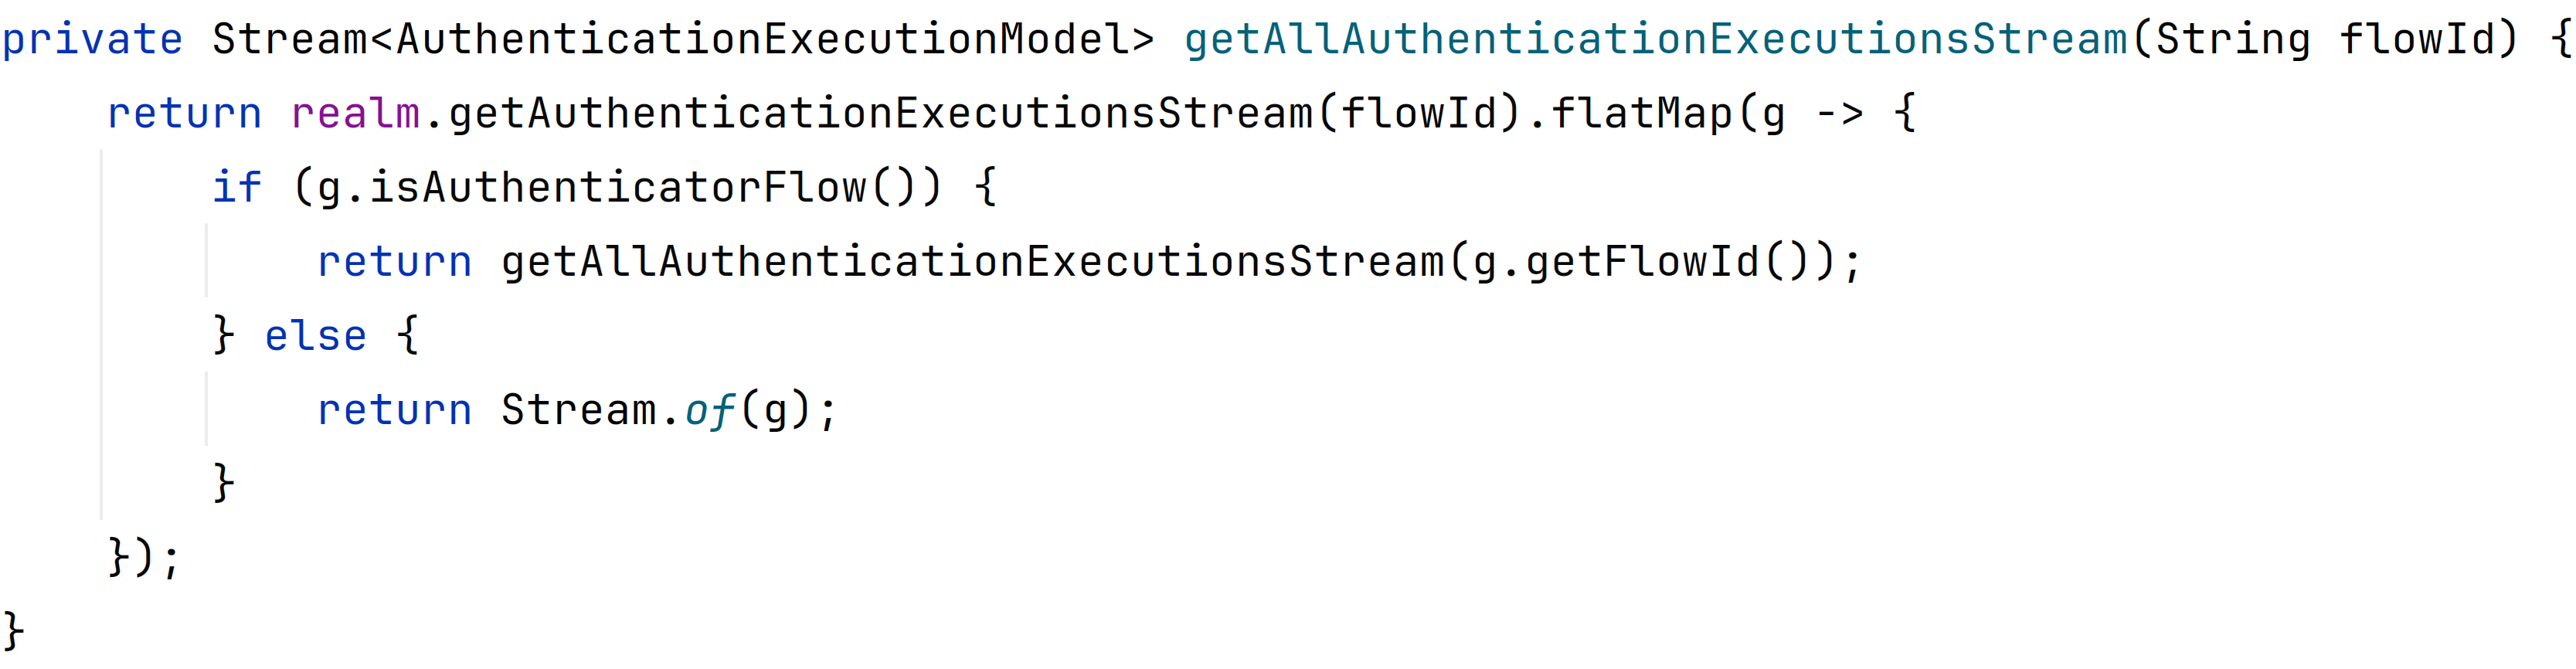
\includegraphics[width=0.95\textwidth]{img/sections/6-implementation/authnPolicyGetAllExecutions.png}
  \caption{Get All Authentication Executions.}
  \label{fig:impl-authn-policies-get-all-execs}
\end{figure}

\newpage
\subsection{REST API} \label{impl-authn-policies-rest}
A REST API (also known as RESTful API) is an API that conforms to the constraints of REST architectural style and allows for interaction with RESTful web services.
REST stands for \textit{REpresentational State Transfer}.\cite{impl-rest} 

A client accessing the REST API through the parent endpoint \textit{/authn-policies} defined for the \textit{AuthnPoliciesResource} request handler class.
When an HTTP request is sent to the endpoint, it is handled by the class, which directs it to the appropriate method based on the HTTP method of the request, shown in Figure \ref{fig:impl-authn-policies-rest}.

The request handler classes work explicitly with the authentication policy DAO, described in Section \ref{impl-authn-policies-dao}.
It provides the isolation of storage operations and user interaction and complies with the Single-responsibility principle.\cite{impl-single-responsibility}

\begin{figure}[htbp]
  \centering
  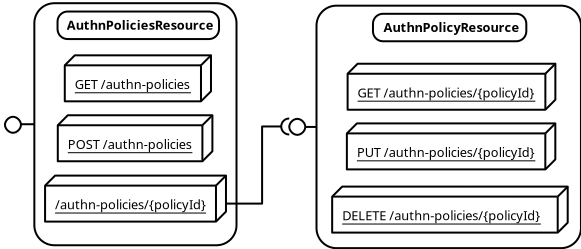
\includegraphics[width=0.9\textwidth]{img/sections/6-implementation/rest.png}
  \caption{Authentication Policies REST API.}
  \label{fig:impl-authn-policies-rest}
\end{figure}

Possible operations on the \textit{AuthnPoliciesResource} request handler class with the additional redirection:
\begin{itemize}
    \item \textit{GET /authn-policies} -- retrieve all authentication policies in JSON format.
    \item \textit{GET /authn-policies/parent} -- retrieve the parent authentication policy in JSON format.
    \item \textit{POST /authn-policies} -- create a new authentication policy with attributes defined as JSON in the request body.  
    \item \textit{/authn-policies/{policyId}} -- Redirects requests to the \textit{AuthnPolicyResource} request handler class.
\end{itemize}

Possible operations on the \textit{AuthnPolicyResource} request handler class:

\begin{itemize}
    \item \textit{GET /authn-policies/\{policyId\}} -- retrieve an authentication policy with ID \textit{policyId} in JSON format.
    \item \textit{PUT /authn-policies/\{policyId\}} -- update an existing authentication policy with ID \textit{policyId} with attributes defined as JSON in the request body.
    \item \textit{DELETE /authn-policies/\{policyId\}} -- delete an existing authentication policy with ID \textit{policyId}.
\end{itemize}

The exact implementation of a specific part of the \textit{AuthnPoliciesResource} class is shown in Figure \ref{fig:impl-authn-policies-rest-impl}.
In the constructor, all necessary initializations are done, and the authentication policy DAO is injected.
When the HTTP request with the \textit{GET} request method is sent to the endpoint, the \textit{getPolicies()} method returns the set of policies in a serialized JSON format.
The abstract model representation is converted to the \textit{Data Transfer Object} (DTO) and returned to the client.

\begin{figure}[htbp]
  \centering
  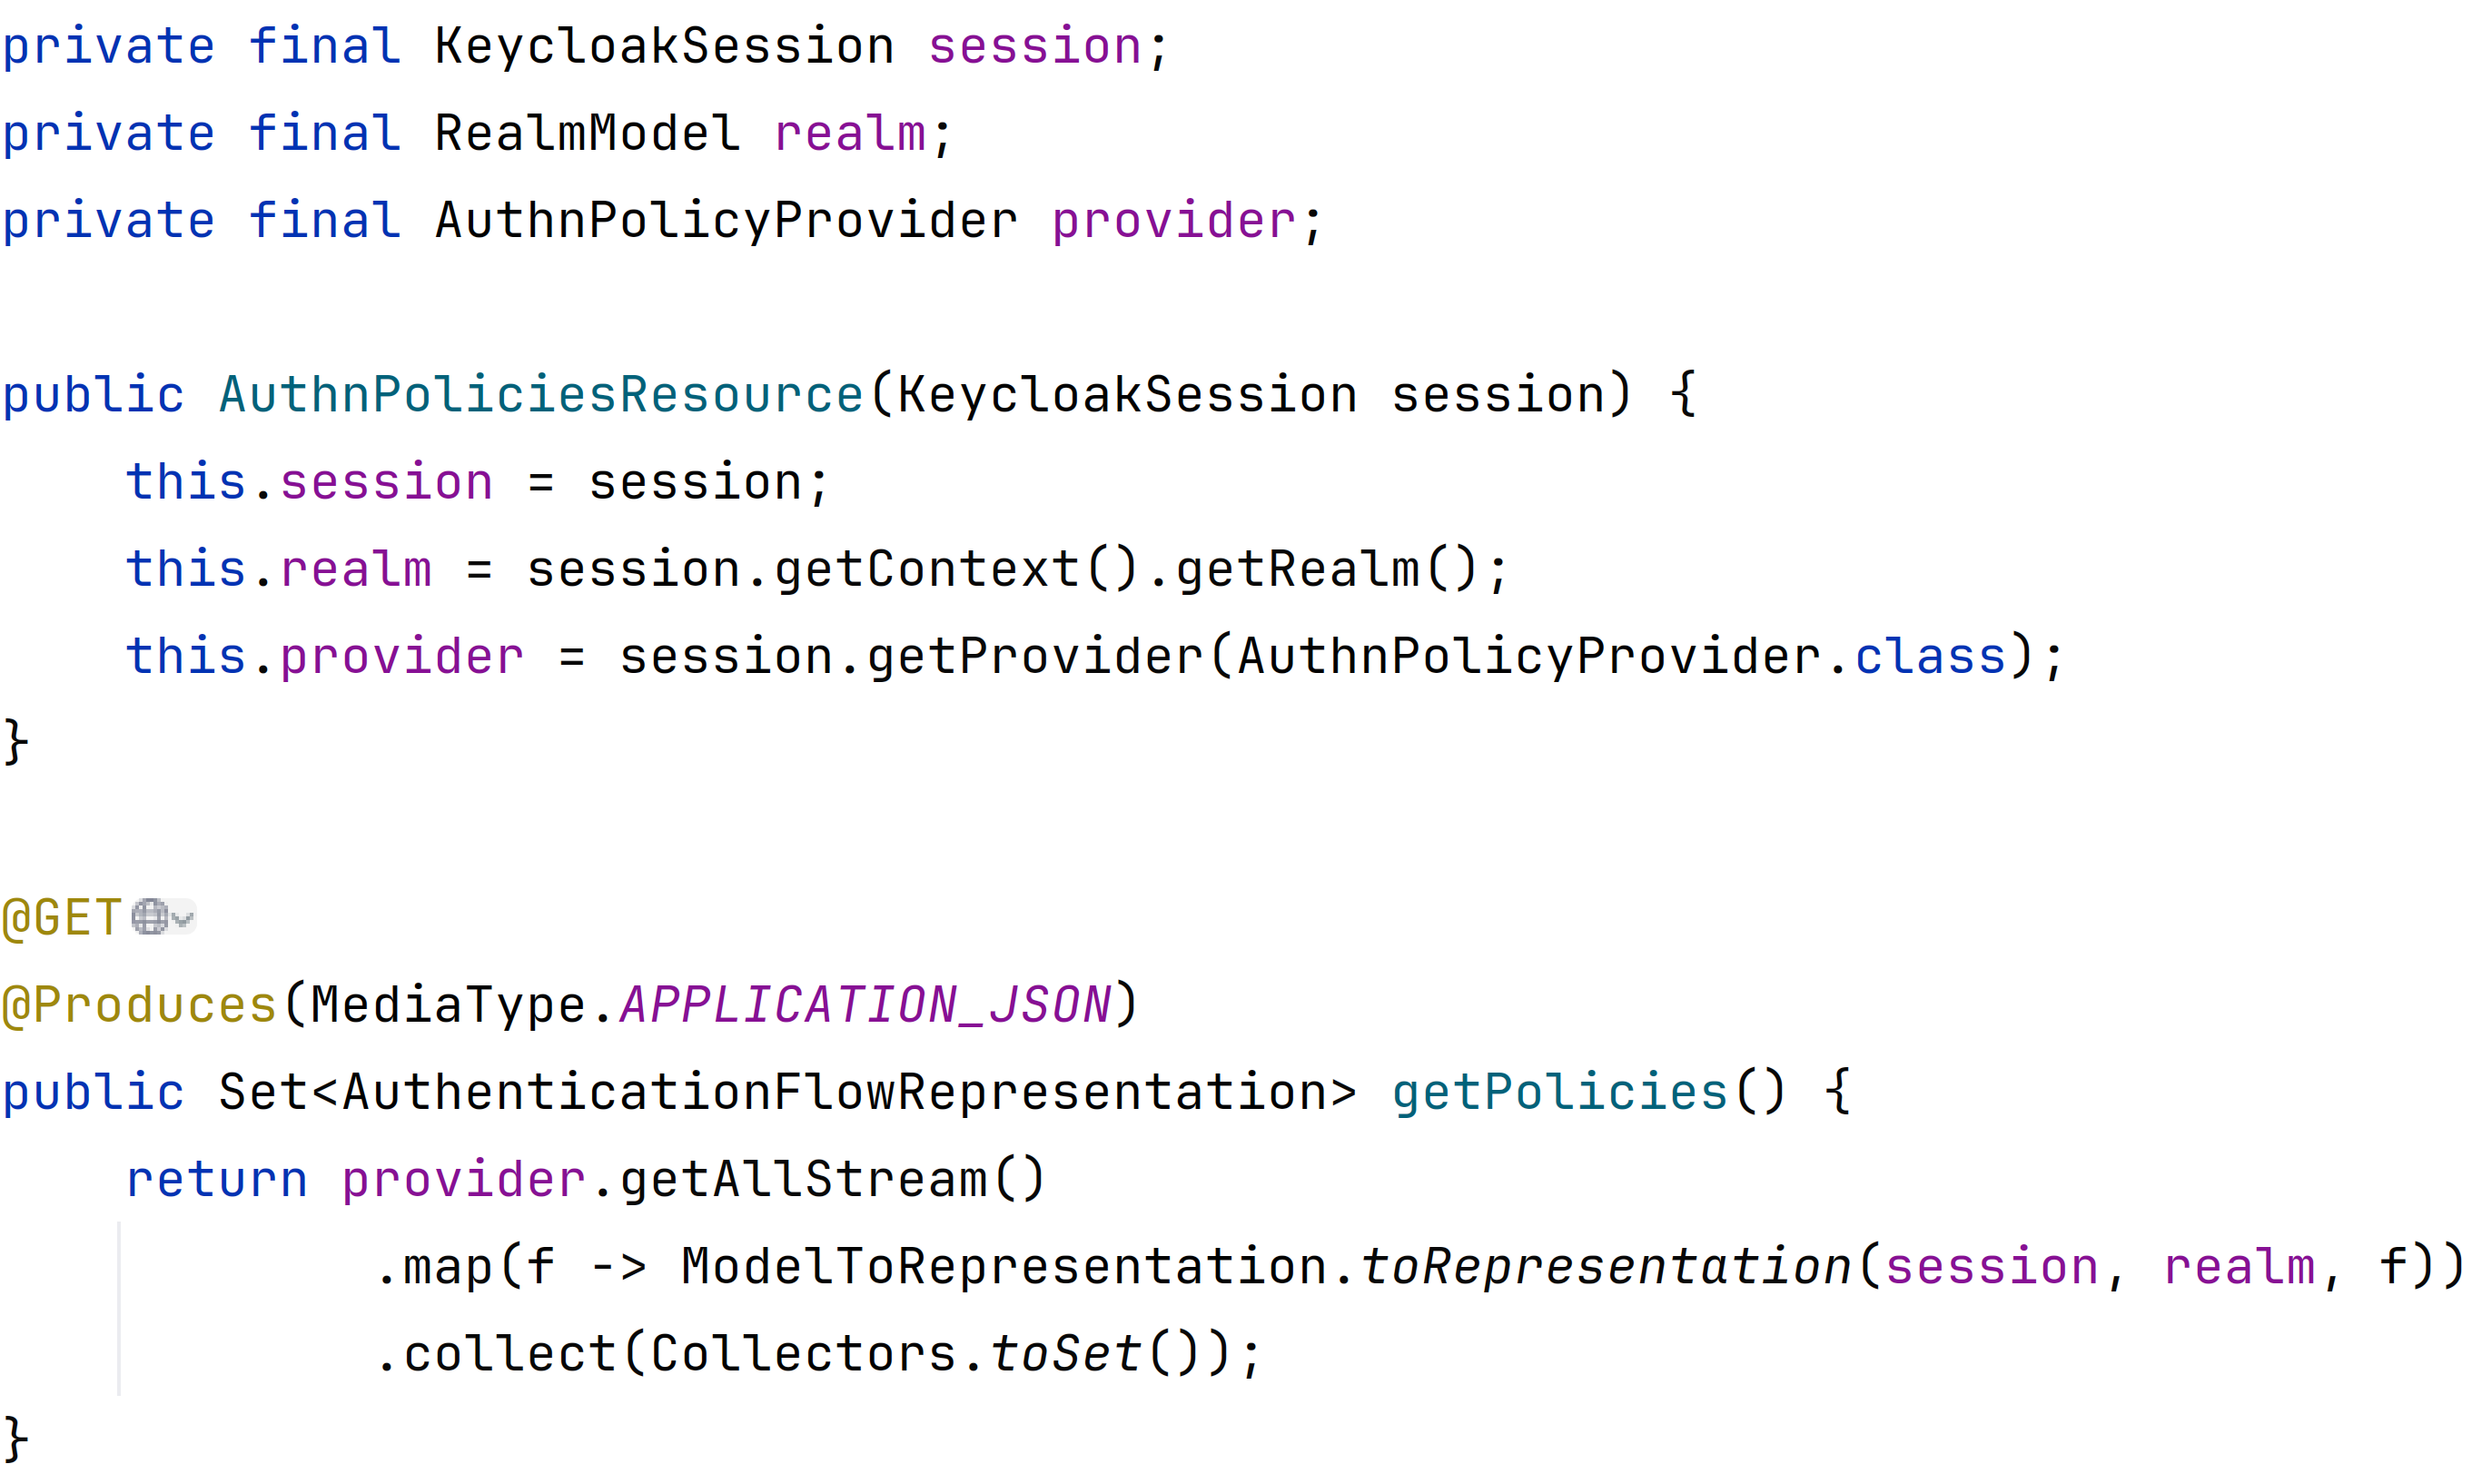
\includegraphics[width=1\textwidth]{img/sections/6-implementation/authn-policy-rest-example.png}
  \caption{Authentication Policies REST API Implementation.}
  \label{fig:impl-authn-policies-rest-impl}
\end{figure}

\newpage
\section{User Context}
The first step for implementing the \textit{UserContext<T>} abstract class is to bind the generic type to the required one, either through extending the abstract class or via a direct reference from the implementation class. 

For demonstration purposes, consider a specific user context \textit{IpProxyContext}, which handles all IP addresses present in the HTTP \textit{Forwarded}, and \textit{X-Forwarded-For} headers used when a proxy is part of the deployment.

The specific \textit{IpProxyContext} was created, shown in Figure \ref{fig:impl-user-ctx-ifc}, in order to bind the type of the user context with a possible extension of it.

\begin{figure}[htbp]
  \centering
  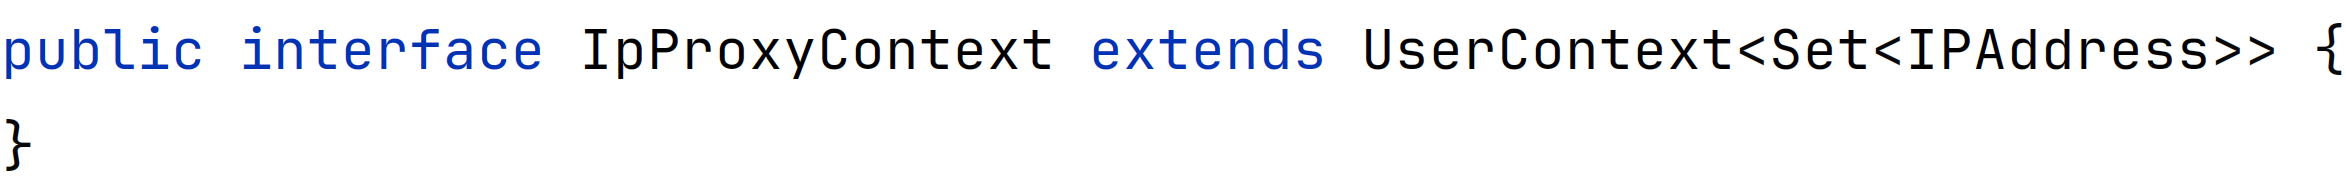
\includegraphics[width=1\textwidth]{img/sections/6-implementation/proxyIpAddressContextInterface.png}
  \caption{Extend \textit{UserContext} Interface.}
  \label{fig:impl-user-ctx-ifc}
\end{figure}

The implementation of the \textit{IpProxyContext}, shown in Figure \ref{fig:impl-user-ctx-ip}, consists of the implementation of the \textit{initData()} method to fulfill the requirements of the abstract class.

With the help of the \textit{KeycloakSession}, the data for a particular context is processed only once per request, so when different risk evaluators need the context, it is not evaluated multiple times.

However, the initialization of the data does not have to be successful.
In that case, the \textit{isInitialized} Boolean flag is \textit{false}, and the user contexts processing unit may repeat the initialization based on the information.

During the initialization of the data, the HTTP headers of the current request are parsed.
IP addresses included in the headers \textit{Forwarded} and \textit{X-Forwarded-For} are concatenated together.
When there is valid data, the Boolean flag \textit{isInitialized} is set to \textit{true}, which notes the initialization is done correctly and data is available. 

\begin{figure}[htbp]
  \centering
  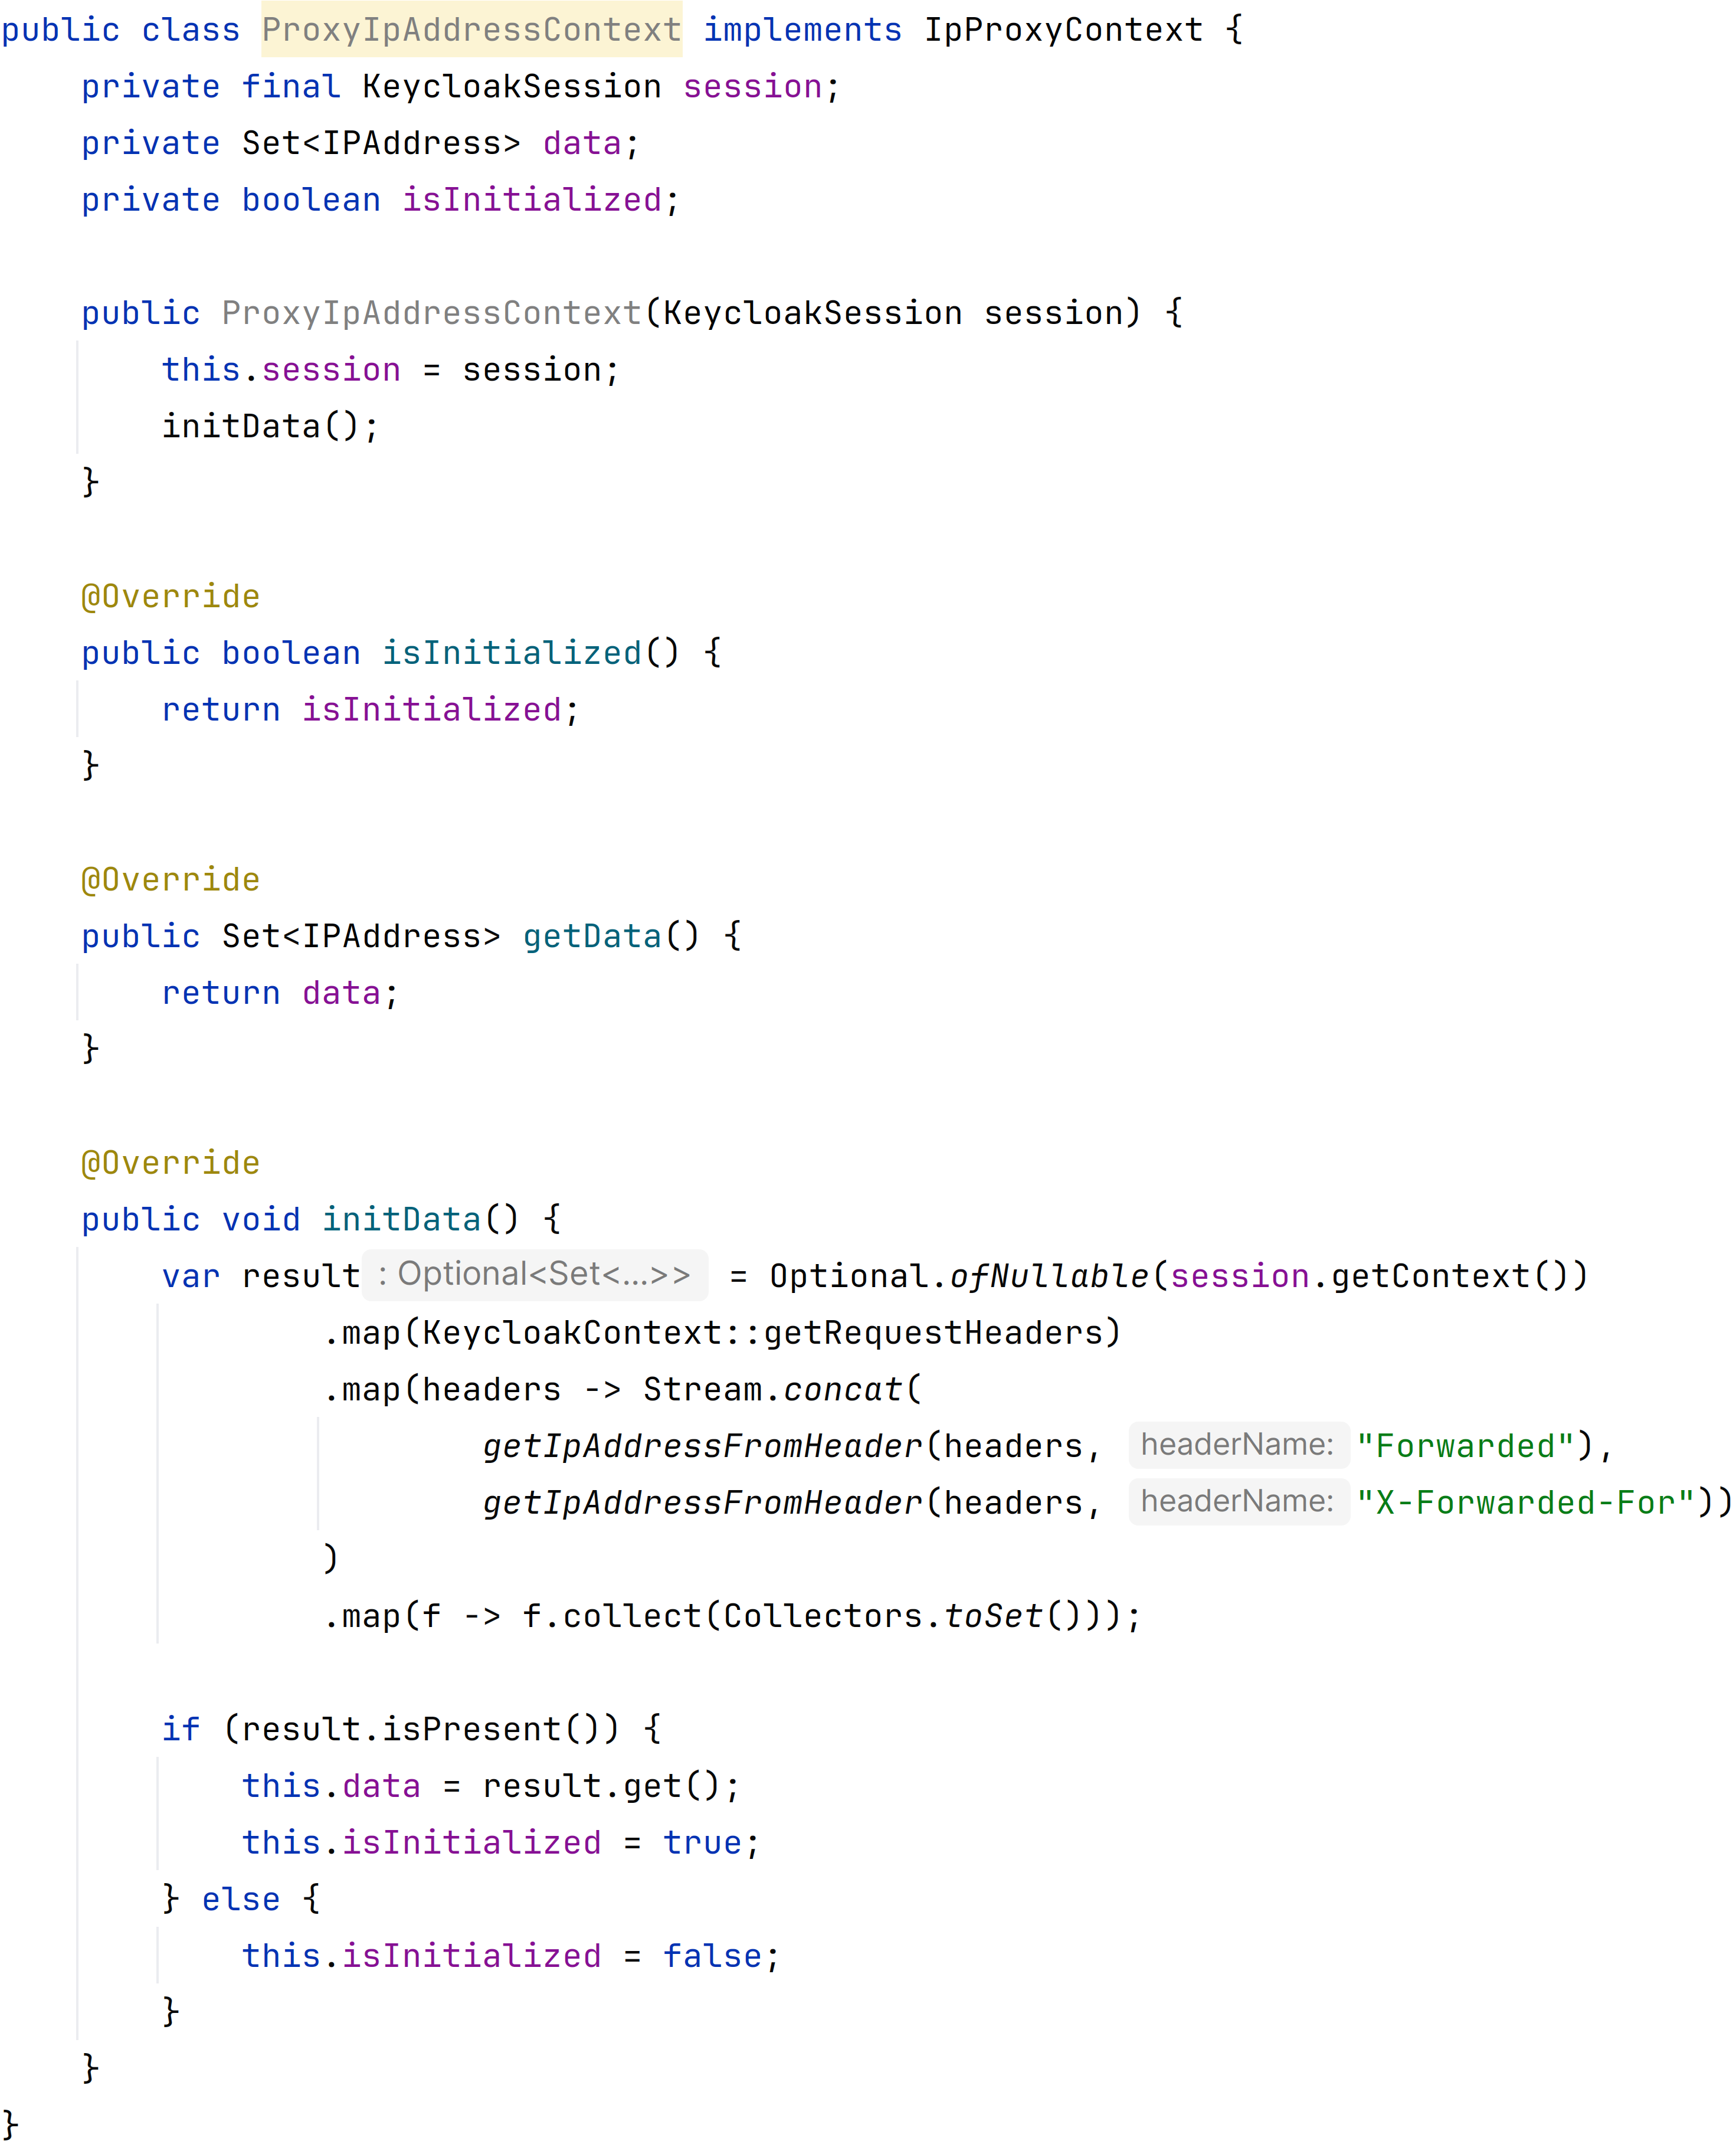
\includegraphics[width=1\textwidth]{img/sections/6-implementation/proxyIpAddress-full.png}
  \caption{Implementation of the \textit{IpProxyContext}.}
  \label{fig:impl-user-ctx-ip}
\end{figure}

\newpage
\section{Risk Evaluator}
A suitable example for the risk evaluator implementation is the specific \textit{LoginFailuresRiskEvaluator}, which statically evaluates the risk based on login failures shown in Figure \ref{fig:impl-risk-evaluator-login-failures}.
For further evaluation, the current IP address is required, so it is obtained from the \textit{IpAddressContext}.

The evaluated risk is returned as \textit{Optional}, as the risk might not be evaluated in time or at all. 
It helps to avoid working with \textit{null} values.
This evaluator requires to have information about the authentication user, so the method \textit{requiresUser()} is amended based on it.

\begin{figure}[htbp]
  \centering
  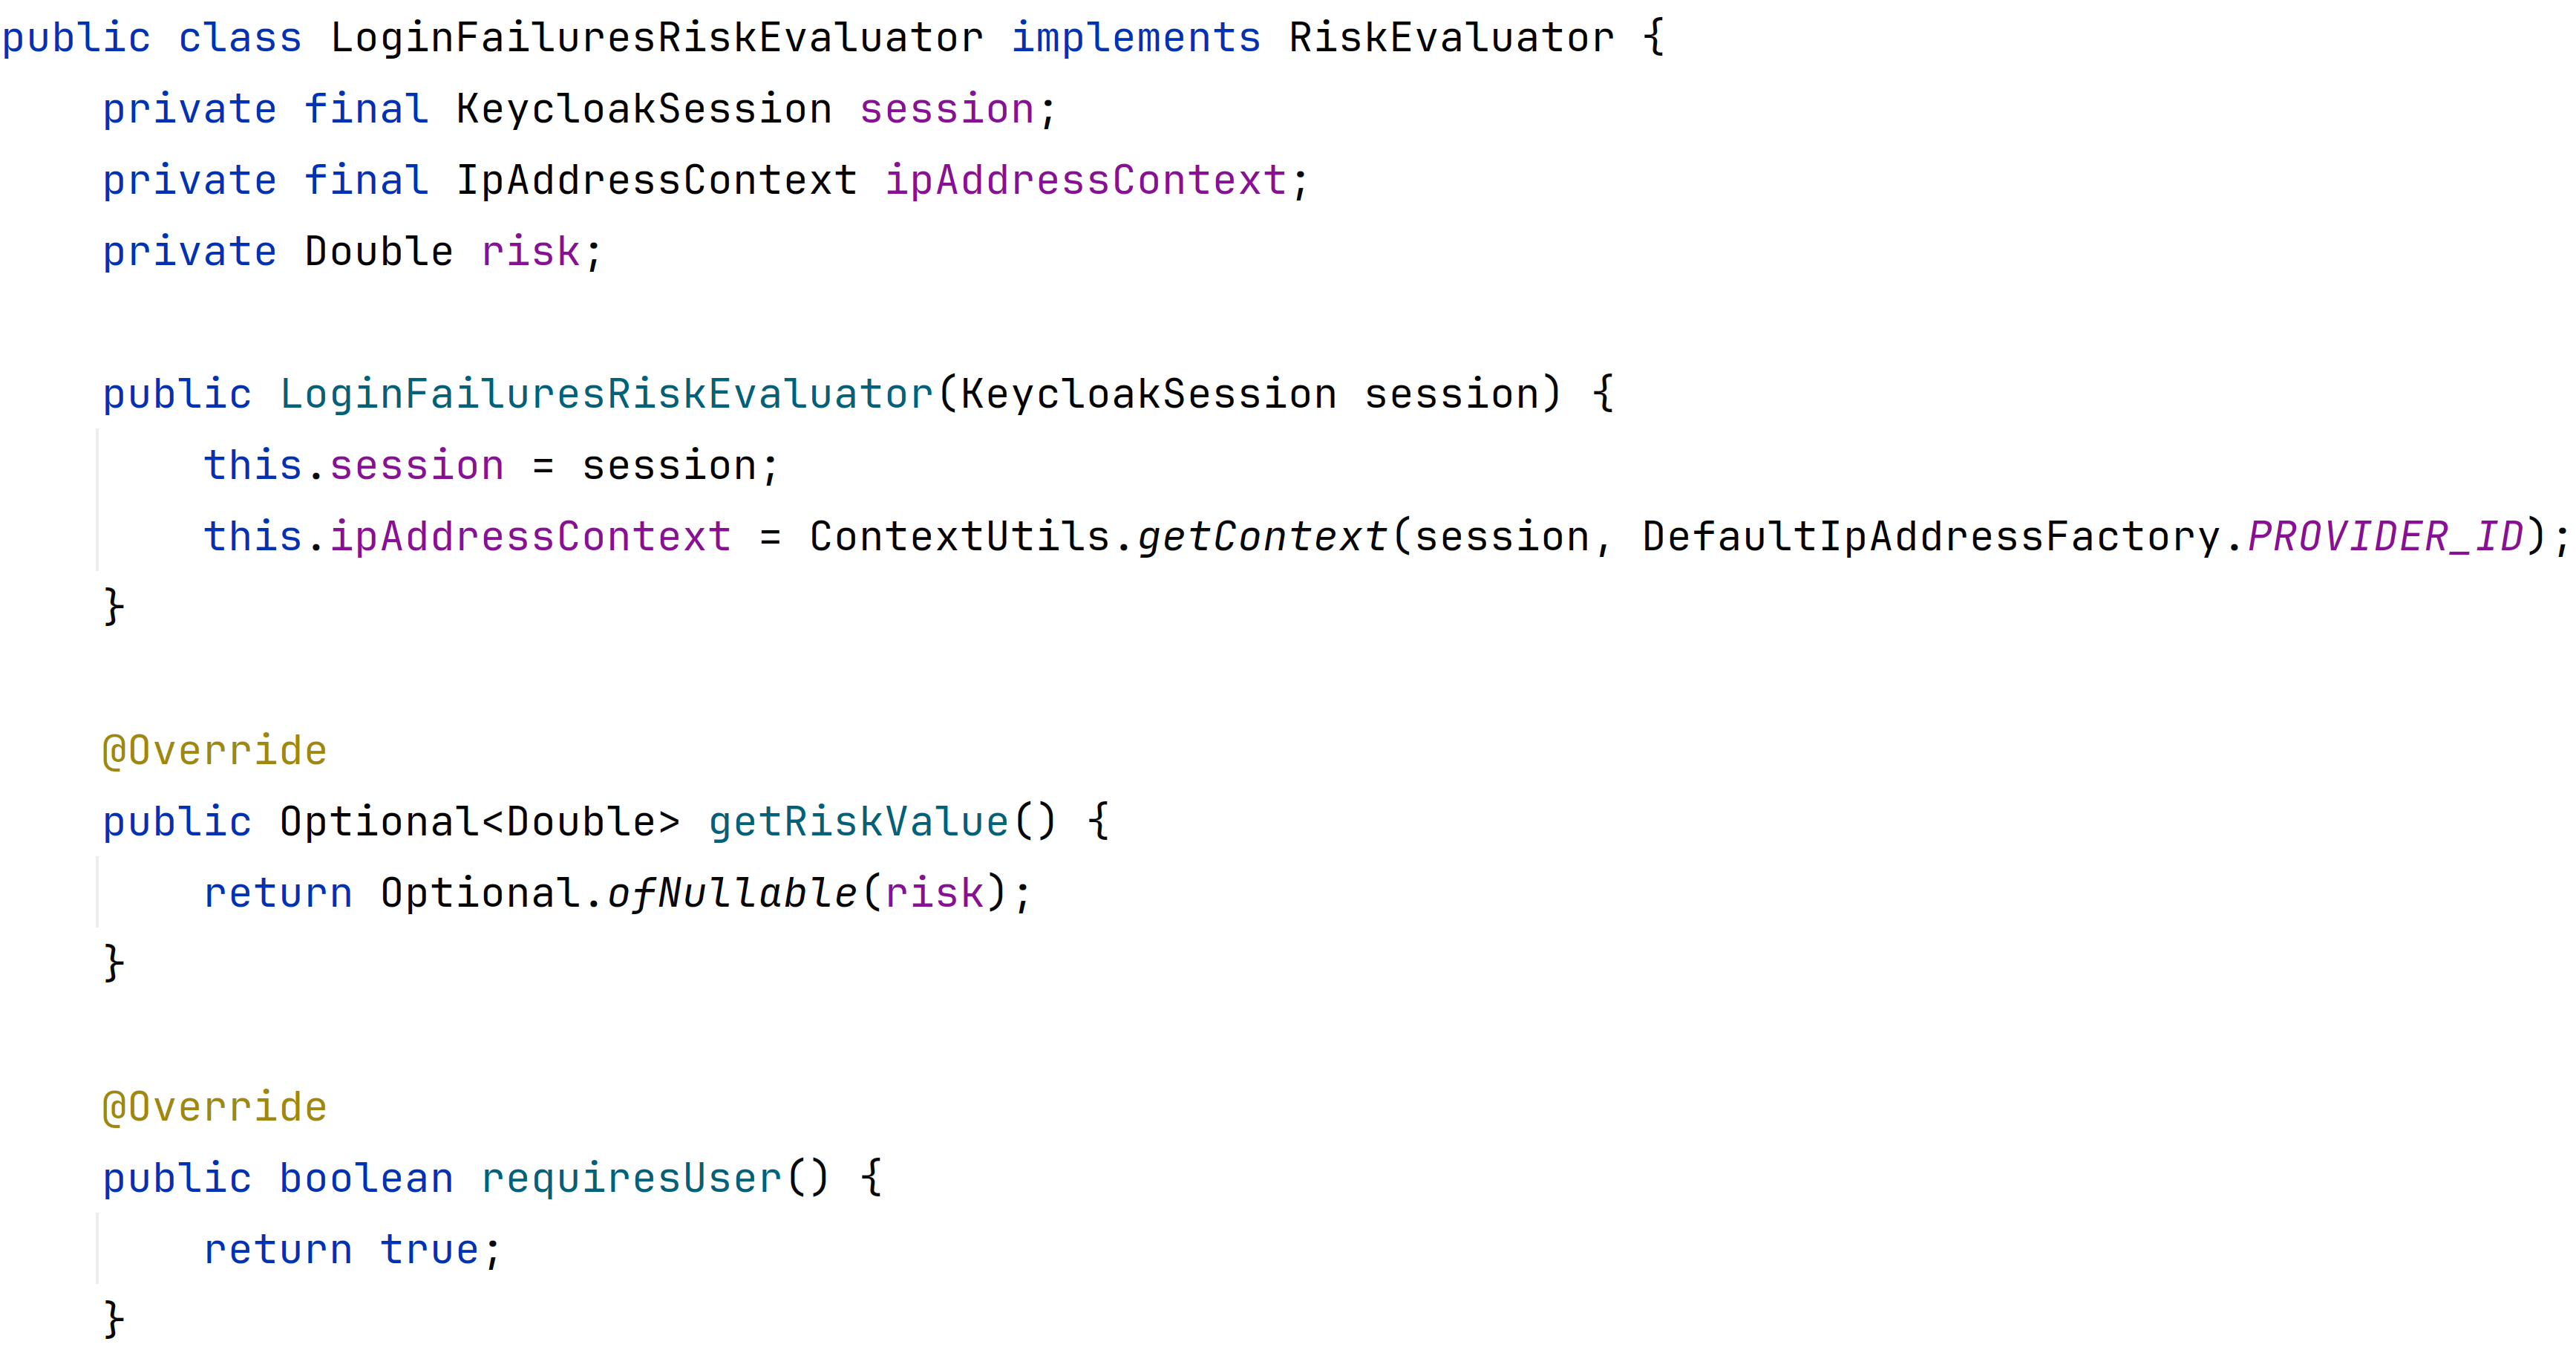
\includegraphics[width=1\textwidth]{img/sections/6-implementation/loginFailures.png}
  \caption{Login Failures Risk Evaluator.}
  \label{fig:impl-risk-evaluator-login-failures}
\end{figure}

The evaluation of the risk itself is done in the \textit{evaluateRisk()} method, which contains a few checks of login failures, as shown in Figure \ref{fig:impl-risk-evaluator-login-failures-evaluations}.
As was mentioned before, the evaluation of the risk itself might be challenging and requires specific agreements on the evaluations, as there is no explicit correct approach to achieving it.

In the example, the risk is increasing based on the count of login failures, which might represent a brute-force attack.
The higher the count of login failures, the higher the risk.

The last check verifies the current IP address and the IP address of the last login failure, as requesting resources from different IP addresses should indicate a higher risk.
There might be a situation where the risk for a legitimate user trying to access the application will be higher, as some fraudulent activity has been executed based on their account. 

\begin{figure}[htbp]
  \centering
  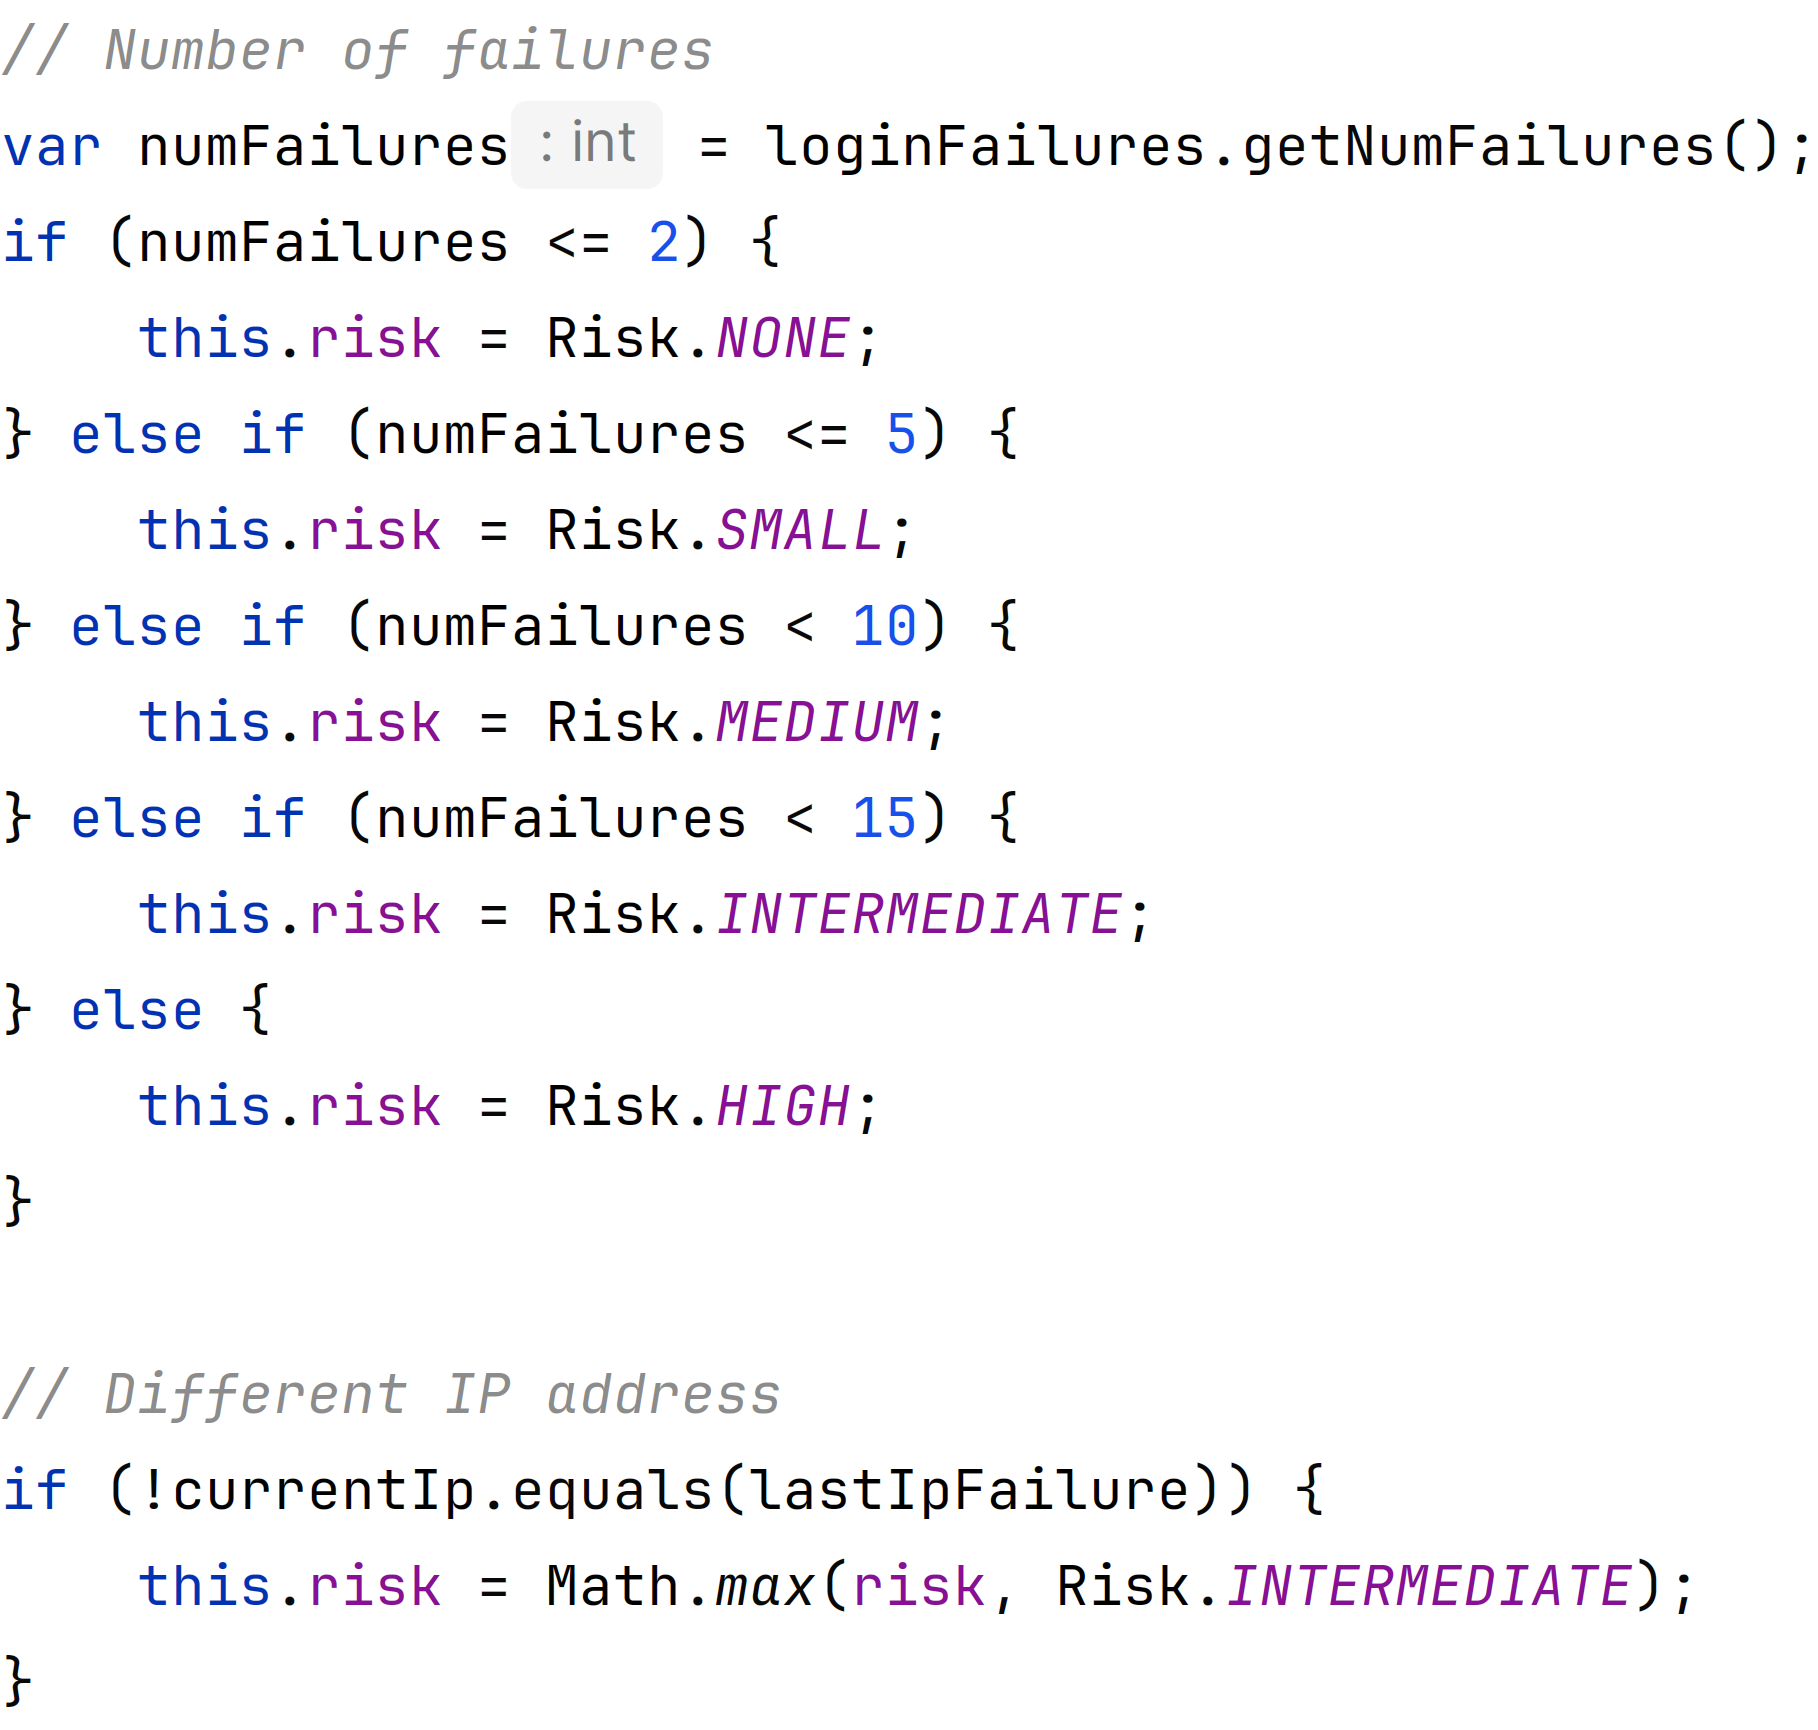
\includegraphics[width=0.7\textwidth]{img/sections/6-implementation/loginFailuresEvals.png}
  \caption{Login Failures Risk Evaluator Evaluations.}
  \label{fig:impl-risk-evaluator-login-failures-evaluations}
\end{figure}

\subsection{Configuration}
By default, for every risk evaluator, attributes \textit{isEnabled} and \textit{weight} can be configured by the administrator, as described in Section \ref{design-risk-eval-config}.
The permanent storing of the configuration of risk evaluators is done via realm attributes, which are represented by a key-value map structure.
Every configurable attribute of the risk evaluator has a unique key that is used to reference it in the map structure.

As shown in Figure \ref{fig:impl-risk-evaluator-login-failures-config}, the attributes are obtained from a different location -- from the realm attributes.
In this case, if the \textit{weight} attribute is not stored yet or not configured by the administrator, the default value \textit{Weight.IMPORTANT} (weight 0.8) is applied.
When the \textit{isEnabled} attribute is not stored or configured, it is turned on by default.

\begin{figure}[htbp]
  \centering
  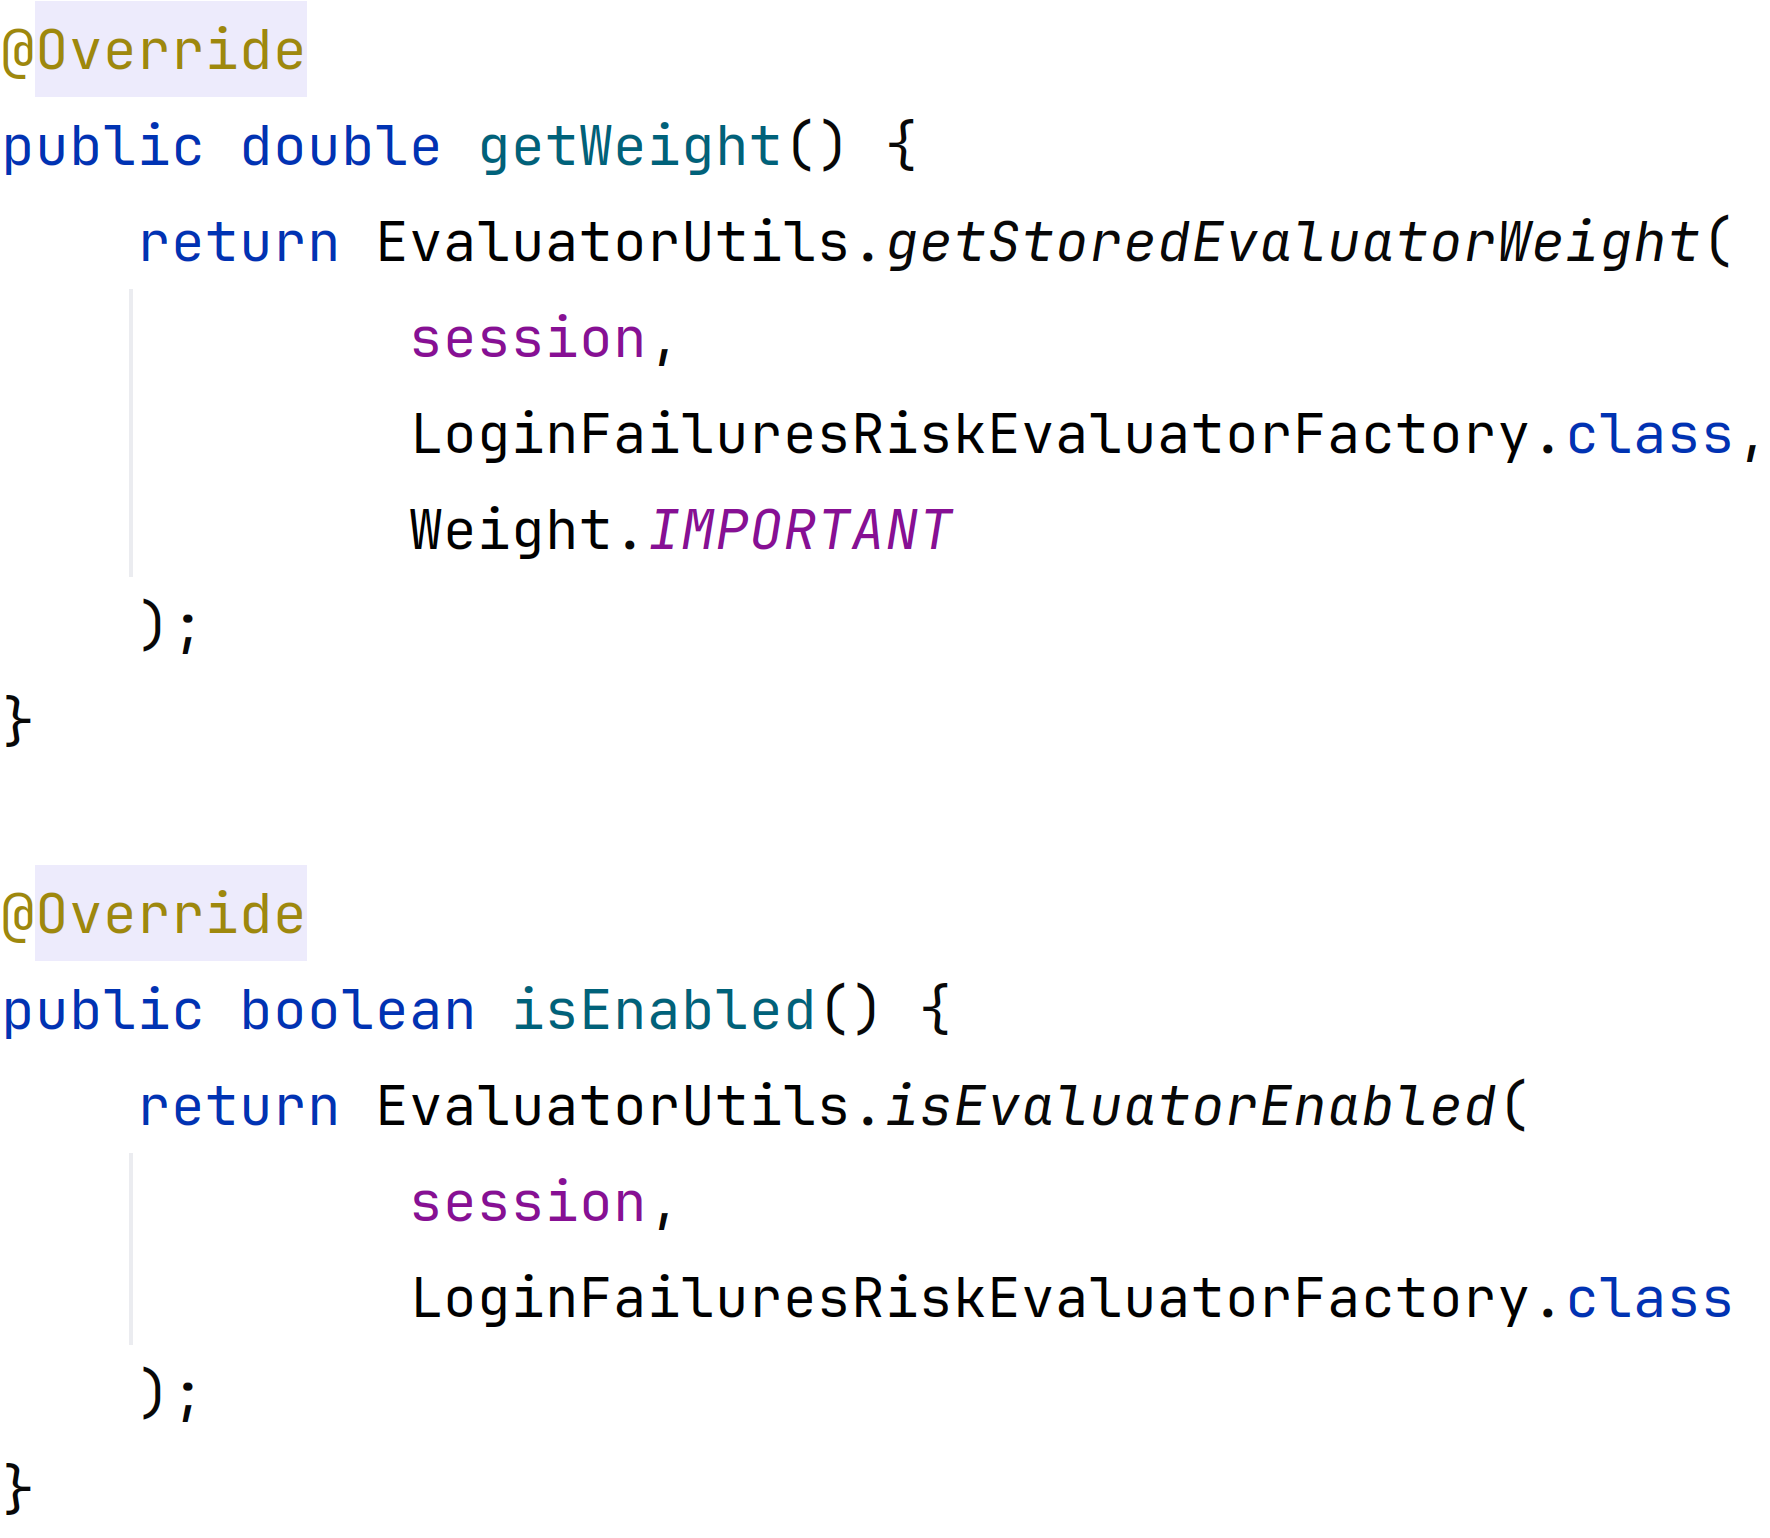
\includegraphics[width=0.6\textwidth]{img/sections/6-implementation/loginFailuresConfig.png}
  \caption{Login Failures Risk Evaluator Configuration.}
  \label{fig:impl-risk-evaluator-login-failures-config}
\end{figure}

\newpage
\section{Risk Engine}

The implementation of the risk engine relies on leveraging \textit{SmallRye Mutiny}
\footnote{https://smallrye.io/smallrye-mutiny/latest/} library to comply with the requirements and design introduced in Section \ref{risk-engine}.
Quarkus officially provides support for the library, and all mentions of the \textit{SmallRye Mutiny} will be primarily focused on the Quarkus Mutiny extension.

The risk engine gathers all risk evaluators, sends a signal to evaluators to start evaluating, retrieves individual scores, and calculates the overall risk score for the authentication process.

In order to improve performance around risk evaluations, an asynchronous approach for the processing has been introduced, as it has minimal impact on the user experience.
For more details, see the Section \ref{impl-engine-async}.

The implementation of the overall risk evaluation is described more in detail in Section \ref{impl-engine-evaluation}, the retry and timeout mechanism in Section \ref{impl-engine-retry} and Section \ref{impl-engine-timeout}.

\subsection{Asynchronous Processing} \label{impl-engine-async}
For the risk engine, the more risk evaluators are considered, the more information about the authentication context can be evaluated.
However, there might be a high number of evaluators, and their processing of them might be resource and time-consuming.
Even the remote evaluators and remote user contexts are considered, so the latency is high, and the current thread is blocked.
Asynchronous processing mitigates these problems.

Asynchronous processing of risk evaluators is provided via the \textit{SmallRye Mutiny} library, in which the main concepts are based on asynchronous message passing and non-blocking \textit{I/O}.

Asynchronous message passing and non-blocking \textit{I/O} are fundamental elements in building responsive, resilient, and efficient distributed systems.
In reactive systems, components communicate asynchronously through message passing, promoting loose coupling in both space and time.

This approach allows systems to handle failures gracefully and adapt to changing conditions.
Quarkus utilizes non-blocking \textit{I/O} to efficiently manage input/output operations, such as database interactions and remote service calls. \cite{quarkus-reactive}

The individual risk evaluations are processed on \textit{I/O} threads, which provides the possibility of using non-blocking \textit{I/O}.
When a remote service is called, the thread is not blocked.
During that case, the \textit{I/O} continuation is scheduled, a continuation is passed, and the thread is released in order to process different tasks.
The continuation is basically a code, which will be executed once the \textit{I/O} is complete.\cite{quarkus-reactive}

As shown in Figure \ref{fig:impl-risk-engine-io-threads}, the evaluator \textit{x} initiates the risk evaluation, and once it starts executing \textit{I/O} operations, the \textit{I/O} continuation is scheduled.
During that, as the thread is released, the evaluator \textit{y} started the risk evaluation.
Once the \textit{I/O} is completed for the evaluator \textit{x}, the continuation is executed.
It utilizes CPU resources as much as possible.
In order to guarantee an upper bound time, the timeout is set so evaluations do not spend more time on evaluations than the specified timeout.

\begin{figure}[htbp]
  \centering
  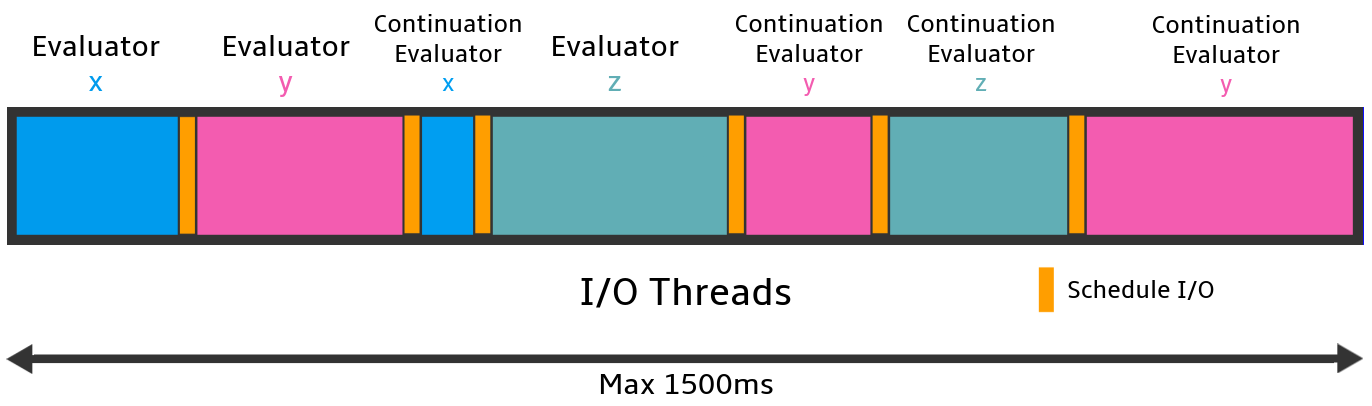
\includegraphics[width=1\textwidth]{img/sections/6-implementation/async.png}
  \caption{\textit{I/O} Threads.}
  \label{fig:impl-risk-engine-io-threads}
\end{figure}

\newpage

\subsubsection{Authentication Flow}
As described in Section \ref{risk-engine}, two categories of risk evaluators are present for the overall risk evaluations based on the user requirements -- ones that require an authentication user and ones that do not.
Consider a simple authentication flow with username and password forms and a risk engine authenticator for the additional authentication executions, as shown in Figure \ref{fig:impl-risk-engine-flow}.

In order to not block the main thread with the risk evaluations that do not require a user, a separate thread is used.
The risk is not needed at that time at all, so it does not have to slow down the authentication process and get a worse user experience.
The dedicated \textit{risk-engine} thread executes tasks for these risk evaluators, leverages the asynchronous processing, and stores the computed overall risk for the particular phase.

The approach for later evaluations of risk evaluators that do require a user is slightly different.
The asynchronous approach is used as well, but the risk engine execution needs to be done on the main thread in a blocking manner.
The reason behind this is the risk engine needs to have valid, correct results for the overall risk evaluation and, based on the used risk level determination, assess the authentication flow.
Therefore, after providing the password, the risk engine authenticator executes risk evaluations, waits for the results, and the authentication flow can proceed.

\begin{figure}[htbp]
  \centering
  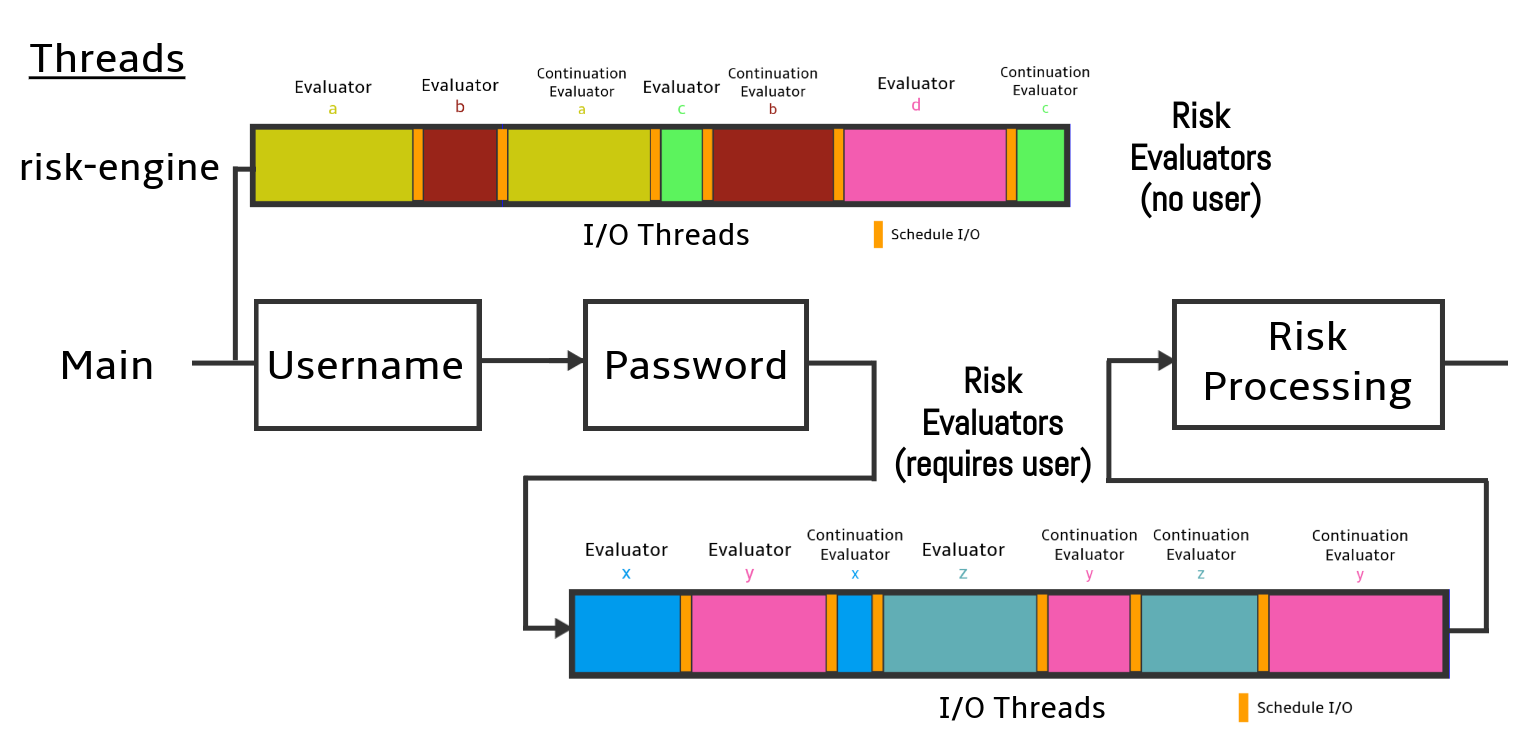
\includegraphics[width=0.95\textwidth]{img/sections/6-implementation/async-flow-final.png}
  \caption{Asynchronous Processing Flow.}
  \label{fig:impl-risk-engine-flow}
\end{figure}

\newpage

\subsection{Retry Evaluations} \label{impl-engine-retry}
Due to unexpected failures, individual risk evaluations might not be properly executed.
During the risk evaluation, either obtaining user contexts or directly the evaluation might fail.
In that case, a retry mechanism has been introduced so the evaluation process is executed again.
The management around retrying risk evaluations handles the risk engine, described in Section \ref{risk-engine}.
The evaluation can be retried at most \textit{n} times, where \textit{n} is the specified \textit{retry} parameter described in Section \ref{risk-engine-config}.
The visual representation of the case is in Figure \ref{fig:impl-risk-engine-retry}.

\begin{figure}[htbp]
  \centering
  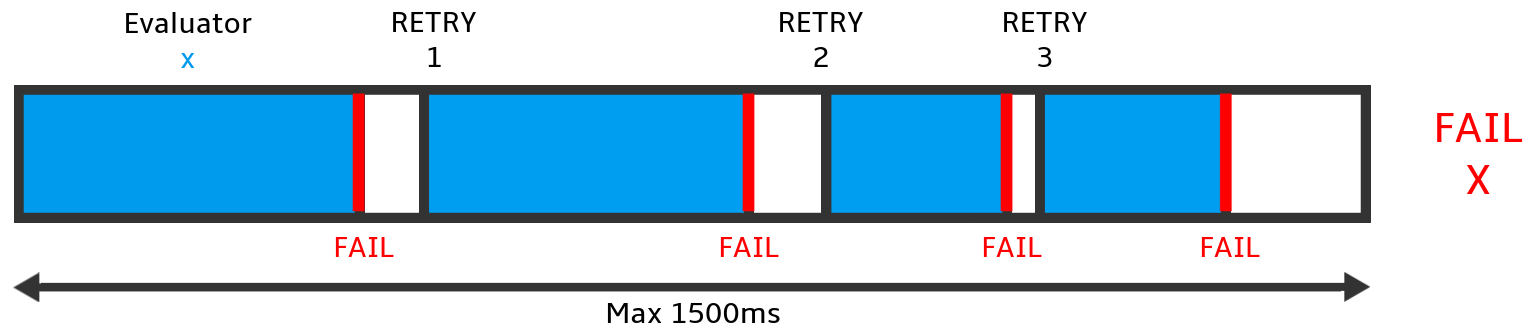
\includegraphics[width=1\textwidth]{img/sections/6-implementation/async-retry.png}
  \caption{Risk Evaluators Retry Mechanism.}
  \label{fig:impl-risk-engine-retry}
\end{figure}

\newpage

\subsection{Evaluations Timeout} \label{impl-engine-timeout}
In order to guarantee specific time boundaries, the timeout for the risk evaluators has been introduced.
It provides the ability to stop risk evaluation after exceeding a specific configurable timeout for a particular risk evaluator.
This means that after exceeding the time limit, the risk evaluator is not taken into consideration for the overall risk score calculations.
For more information about the configuration, see Section \ref{risk-engine-config}.
The visual representation of the case is in Figure \ref{fig:impl-risk-engine-timeout}.

\begin{figure}[htbp]
  \centering
  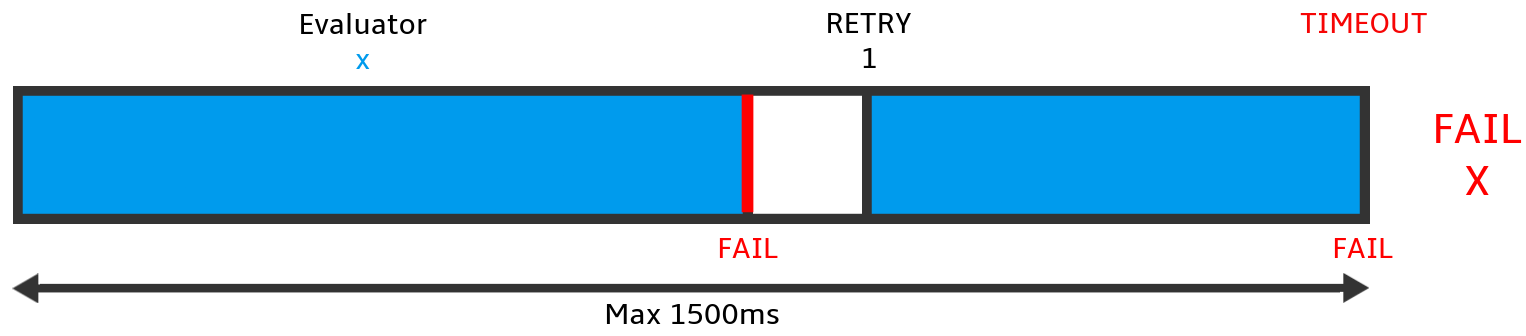
\includegraphics[width=1\textwidth]{img/sections/6-implementation/async-timeout.png}
  \caption{Risk Evalutors Timeout.}
  \label{fig:impl-risk-engine-timeout}
\end{figure}

\subsection{Evaluation} \label{impl-engine-evaluation}
The overall risk score evaluation made by the risk engine leverages the weighted arithmetic mean algorithm, which is the default one, as described in Section \ref{risk-engine-algo}.
When all risk evaluators complete the evaluation, results are collected, and the algorithm is applied, as seen in code snippet \ref{fig:impl-risk-engine-evaluation}.

First of all, for every risk evaluator, the weighted risk score is calculated as \( risk * weight \).
All of these results contribute to the overall weighted risk score summation, which represents the numerator of the algorithm equation.
To obtain a denominator of the algorithm equation, all risk evaluator weights are aggregated and summed together.

After retrieving these two parts of the fraction, the overall risk is calculated and stored for the risk level determination. 

\begin{figure}[htbp]
  \centering
  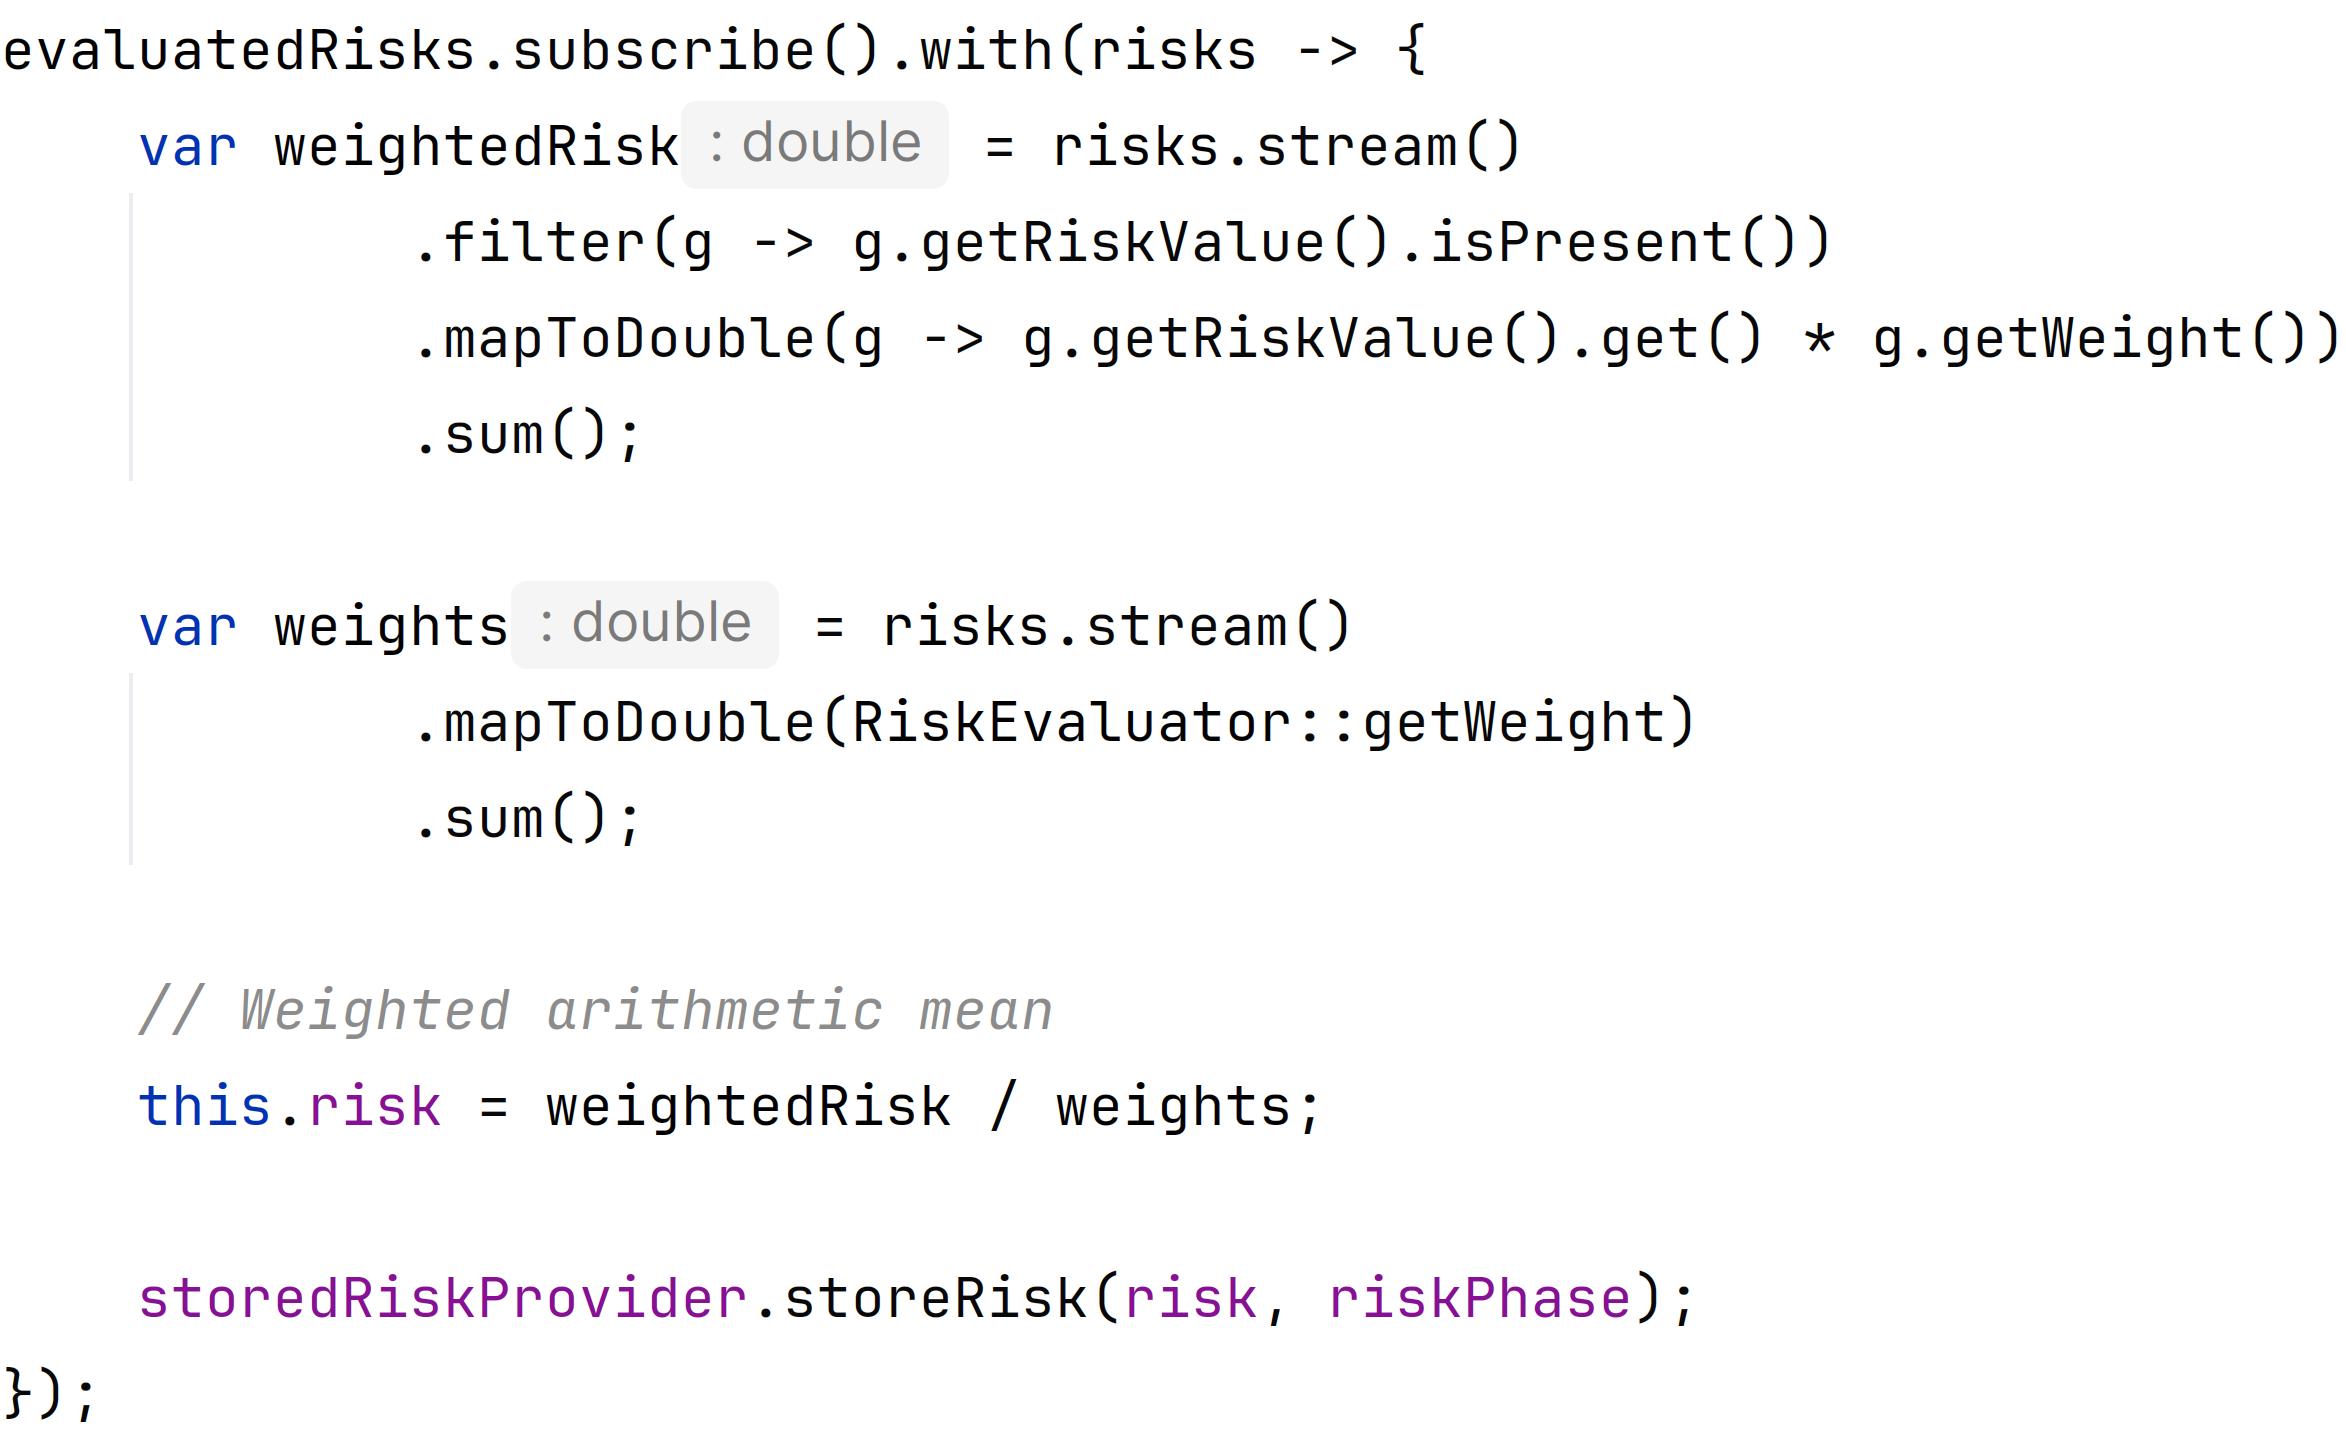
\includegraphics[width=1\textwidth]{img/sections/6-implementation/risk-engine-evaluation.png}
  \caption{Risk Engine Evaluation.}
  \label{fig:impl-risk-engine-evaluation}
\end{figure}

\newpage
\section{Artificial Intelligence}
The implementation of AI relies on the Natural Language Processing (NLP) engine, as described in Section \ref{design-ai}.
The main purpose of integrating AI into risk-based authentication is for individual risk evaluations.

The default NLP engine is ChatGPT, developed by OpenAI as its popularity rapidly grows and meets all requirements of this thesis.
OpenAI provides a REST API for communication with the ChatGPT service, so the integration is seamless.
\newline
\newline
As described in Section \ref{design-ai}, the most important properties of the AI NLP engine are:

\begin{itemize}
    \item \textit{context} -- general context for the AI NLP engine to understand the overall meaning and defining role and scope.
    \item \textit{message} -- specific description of the task.  
\end{itemize}

\begin{figure}[htbp]
  \centering
  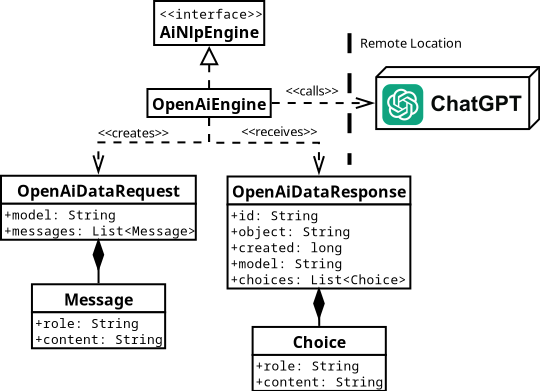
\includegraphics[width=0.85\textwidth]{img/sections/6-implementation/ai-engine-openai.png}
  \caption{OpenAI Integration.}
  \label{fig:impl-ai-openai-integration}
\end{figure}

\newpage

As seen in Figure \ref{fig:impl-ai-openai-integration}, the \textit{OpenAiEngine} implements the \textit{AiNlpEngine} interface and manages the request and response data.
ChatGPT API requires specific data to be provided in order to comply with the API.
\textit{OpenAiEngine} creates the \textit{OpenAiDataRequest} object, which represents request data sent to the API.

The \textit{context} and \textit{message} properties are passed to the request data as \textit{Message} objects.
The \textit{context} property is represented as \textit{Message} object with role \textit{system} and content \textit{context}.
The \textit{message} property is represented as \textit{Message} object with a role \textit{user}, and content \textit{message}.
The data for evaluating risk score are represented as a JSON object with properties \textit{risk} and \textit{reason}, as explained in Figure \ref{fig:impl-ai-context-message}.

\newpage

The default context for evaluating risk score with all necessary information about tasks, boundaries, and format of the result might be as in Figure \ref{fig:impl-ai-context-message}.

\begin{figure}[htbp]
  \centering
  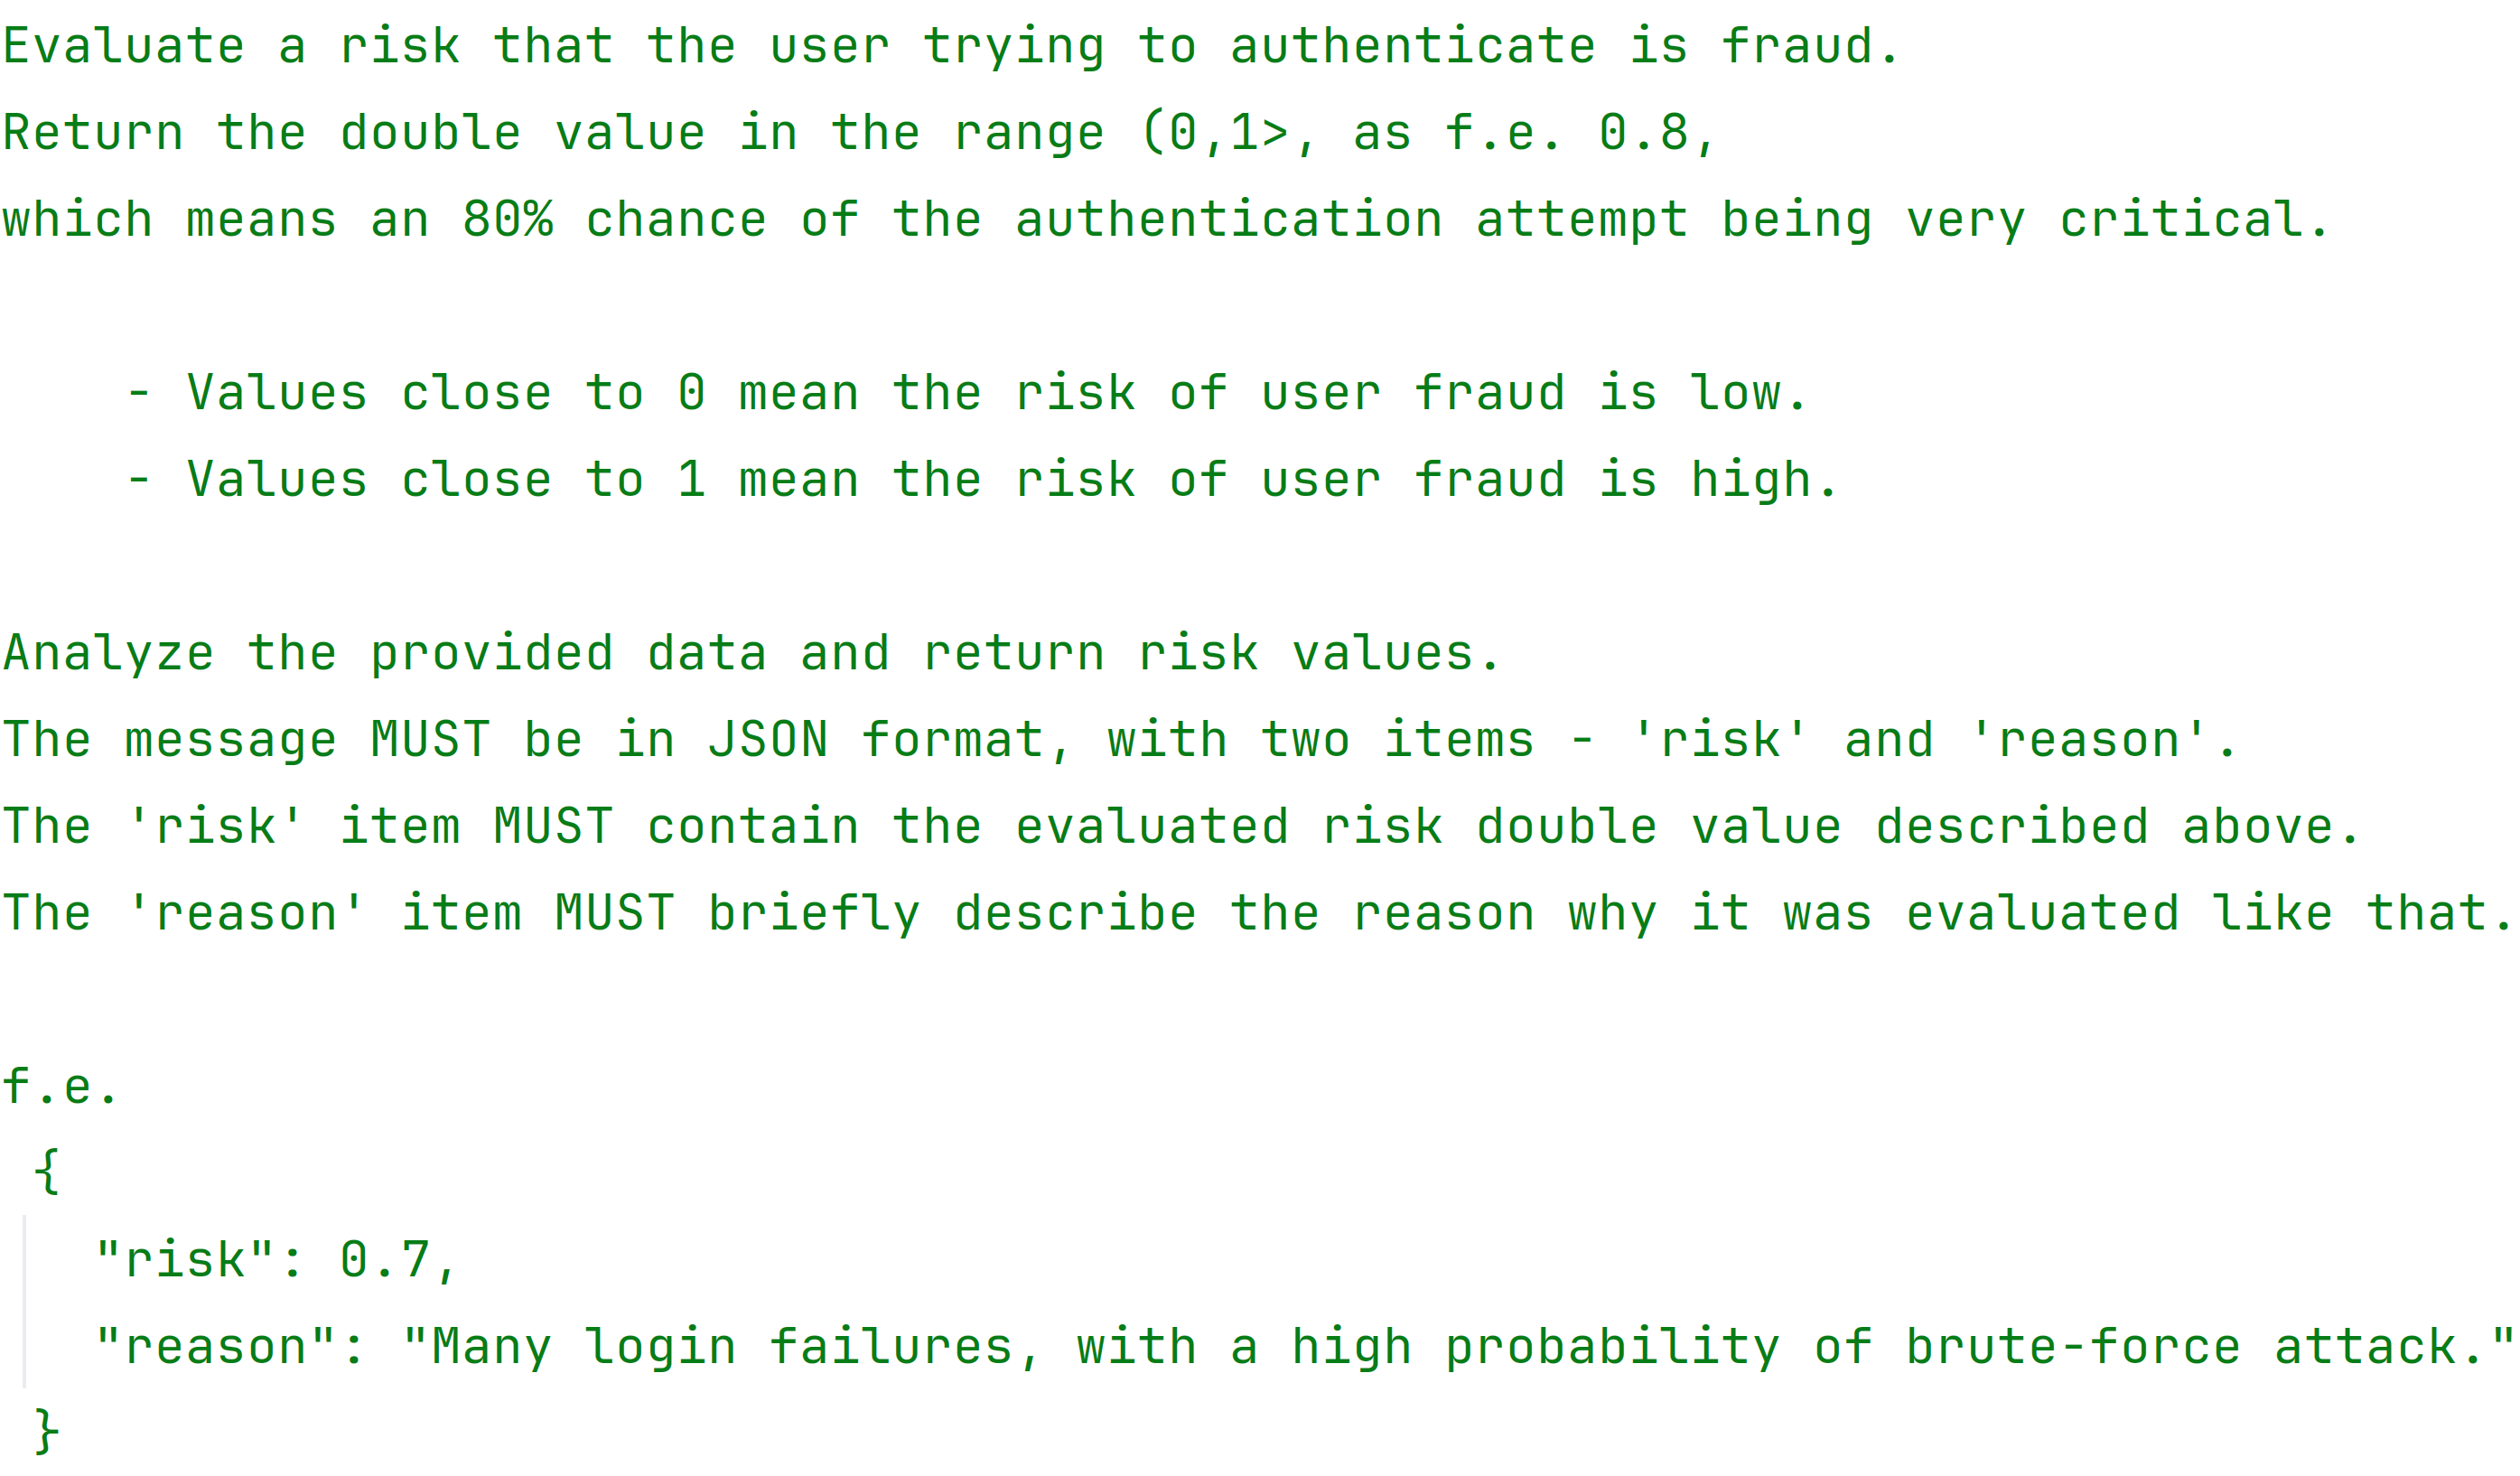
\includegraphics[width=1\textwidth]{img/sections/6-implementation/aiContextMessage.png}
  \caption{AI NLP Context Message.}
  \label{fig:impl-ai-context-message}
\end{figure}

Specific tasks for AI-based risk evaluators contain a dynamically created message with all necessary information for a device representation, as seen in Figure \ref{fig:impl-ai-device-message}. 

\begin{figure}[htbp]
  \centering
  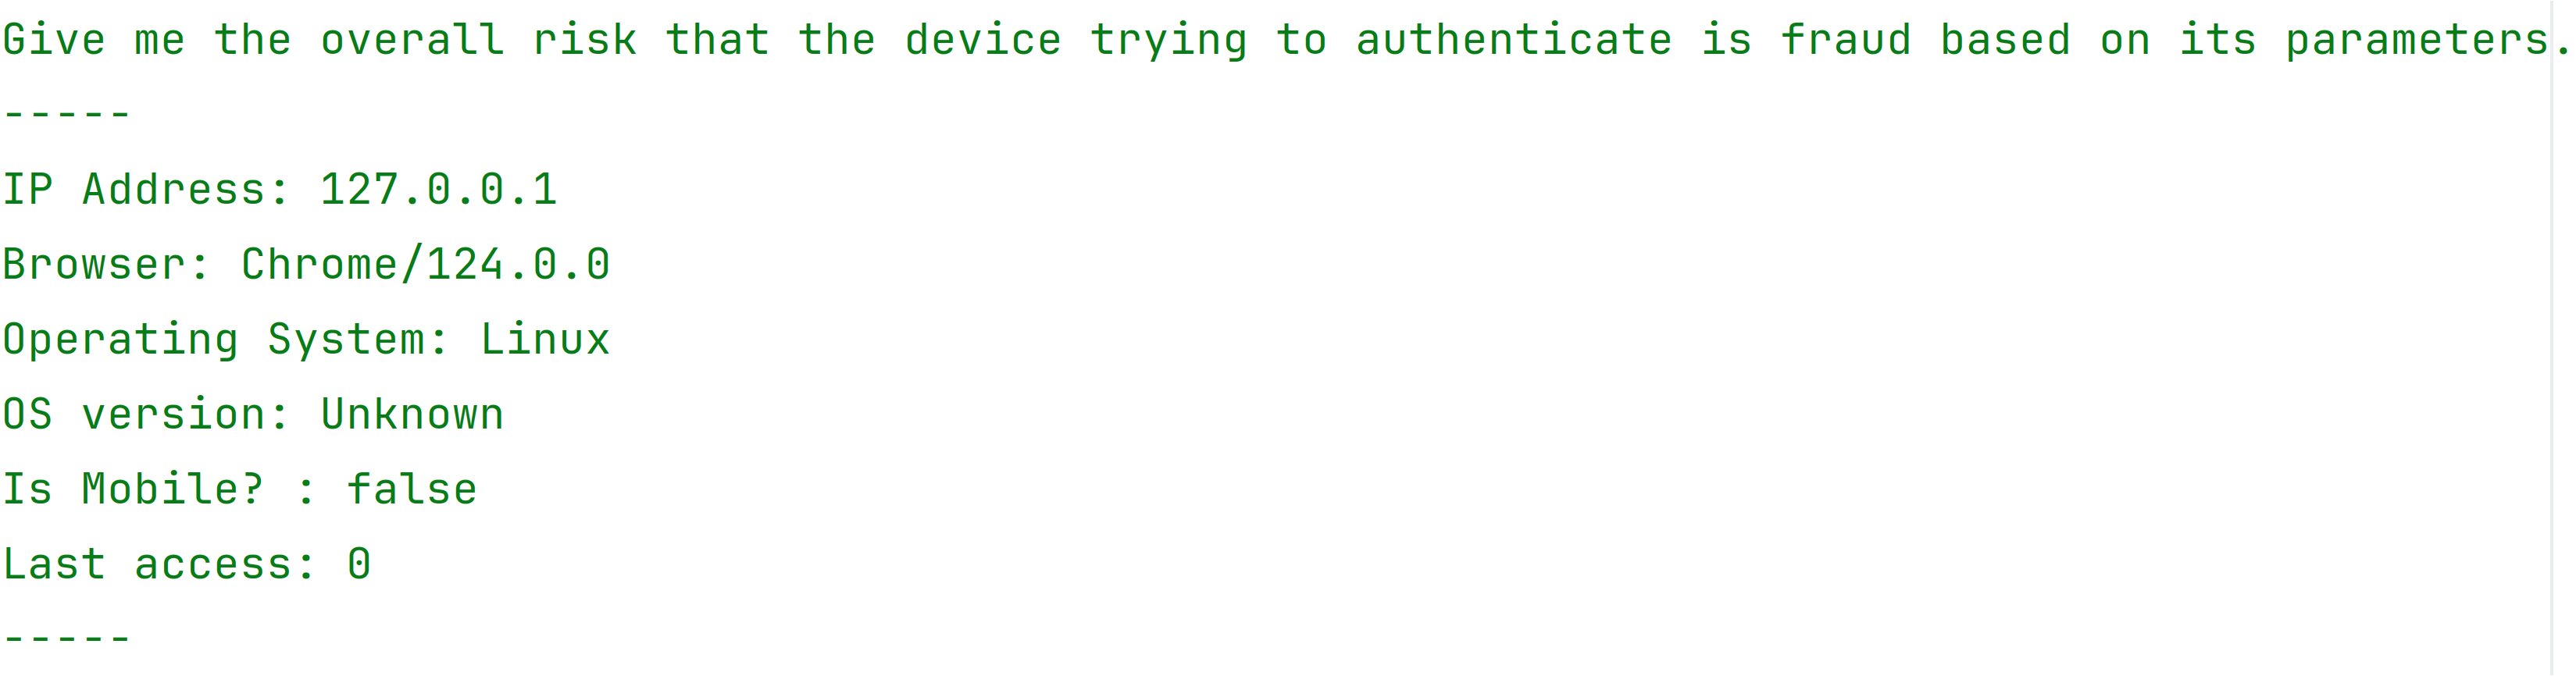
\includegraphics[width=1\textwidth]{img/sections/6-implementation/aiDeviceUserMessage.png}
  \caption{AI NLP Device Query.}
  \label{fig:impl-ai-device-message}
\end{figure}

\newpage

The response from the ChatGPT contains the required data with the specific risk score and the explanation of the reason why it was evaluated like that, as seen in Figure \ref{fig:impl-ai-device-message-response}.

\begin{figure}[htbp]
  \centering
  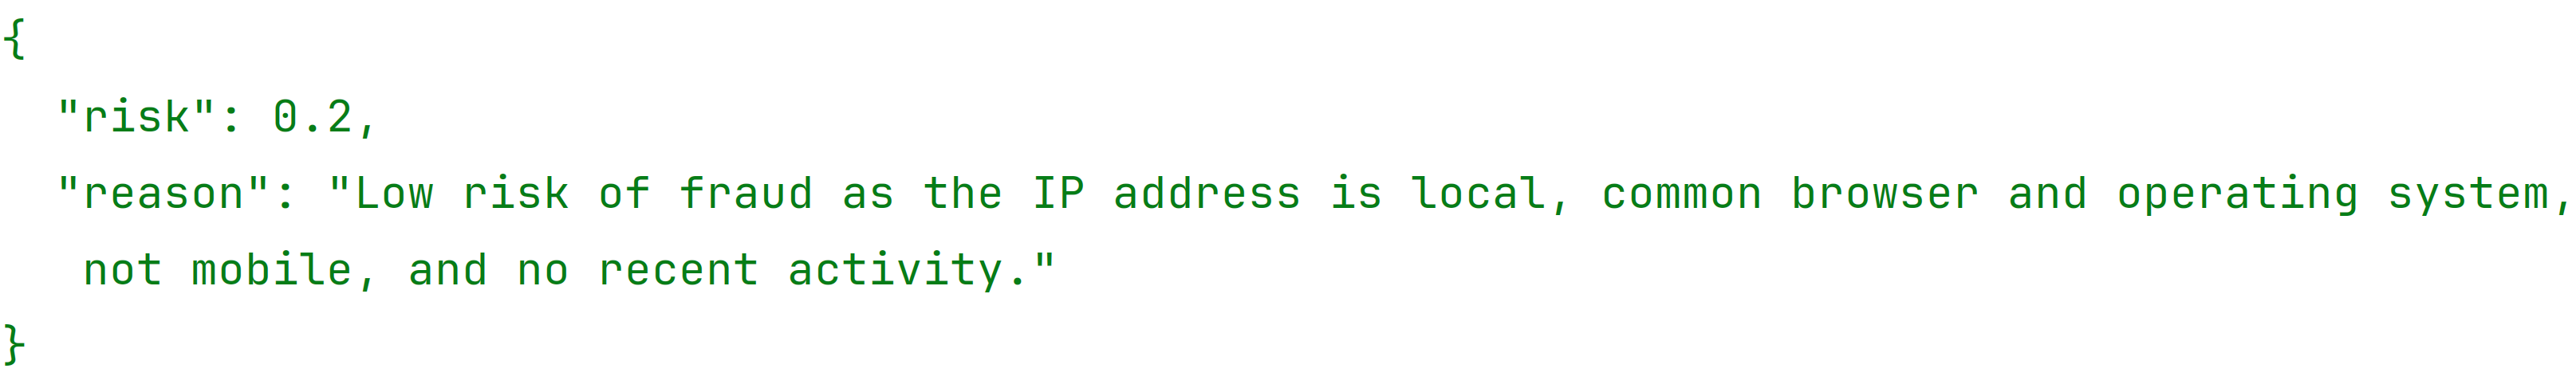
\includegraphics[width=1\textwidth]{img/sections/6-implementation/aiDeviceResponse.png}
  \caption{ChatGPT Device Response.}
  \label{fig:impl-ai-device-message-response}
\end{figure}

The other example is related to evaluating login failures with the user \textit{message}, as seen in Figure \ref{fig:impl-ai-login-message}.

\begin{figure}[htbp]
  \centering
  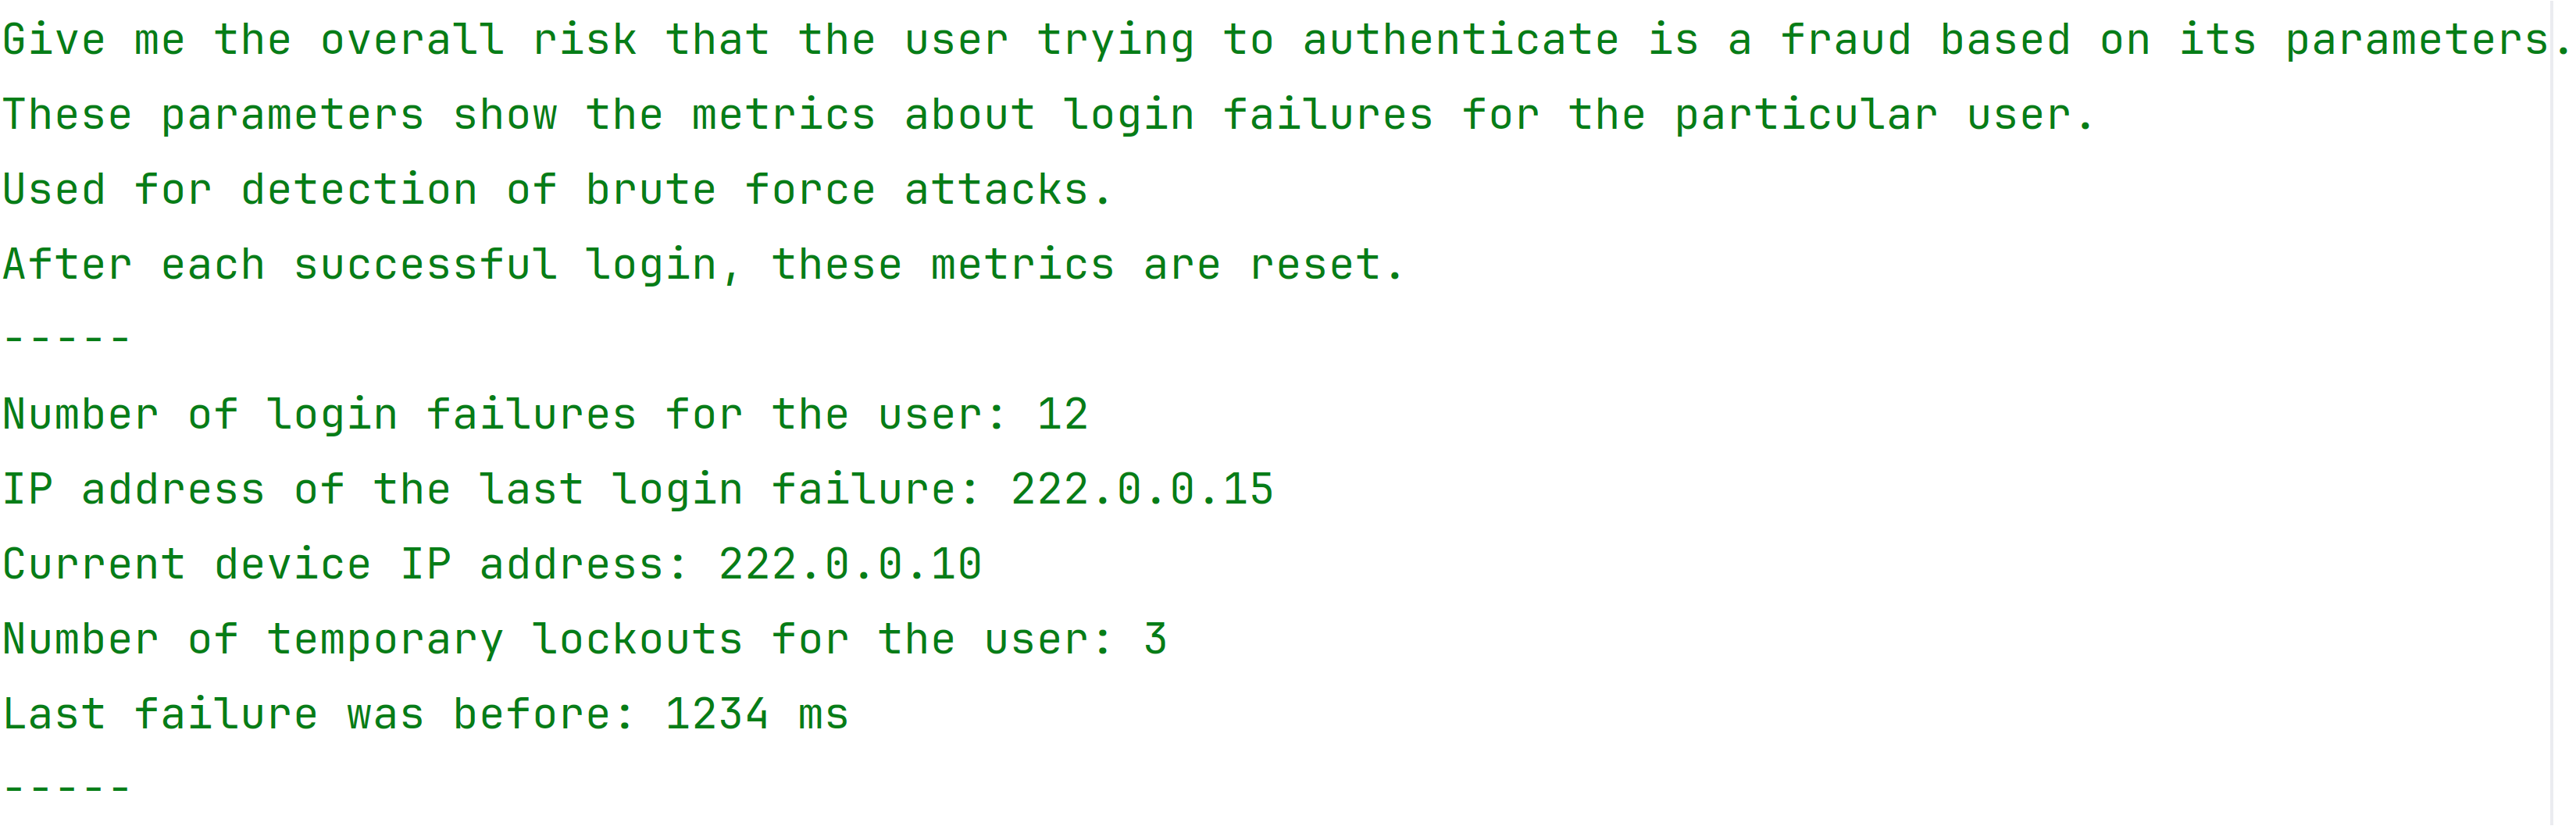
\includegraphics[width=1\textwidth]{img/sections/6-implementation/aiLoginFailureMessage.png}
  \caption{AI NLP Login Failures Query.}
  \label{fig:impl-ai-login-message}
\end{figure}

\section{External Integration}
To demonstrate the external integration with third-party services, the external location user context has been introduced.
As described in Section \ref{design-external-integration}, it is possible to obtain remote user context of arbitrary type.
Obtaining more comprehensive information about the location of the authentication device might be challenging and requires the incorporation of services concentrated on it.
Therefore, retrieving location information from the remote service is suitable for demonstrating external integration with services. 

\newpage

For this purpose, the \textit{ipapi}\footnote{https://ipapi.com/} service is used as it provides a simple API for location information based on the provided IP address.
Remote calls on the service are executed during the initialization of the \textit{IpApiLocationContext} when the IP address from the \textit{IpAddressContext} is returned and substituted to the request.

The approach for the request assembly is straightforward and uses only path parameters of the URL as follows:
\textit{https://ipapi.co/<ip-address>/json}.
The data in the format specified in \textit{IpApiLocationData} class is returned.
The simplified architecture of the \textit{IpApiLocationContext} context is shown in Figure \ref{fig:impl-external-ipapi}.

\begin{figure}[htbp]
  \centering
  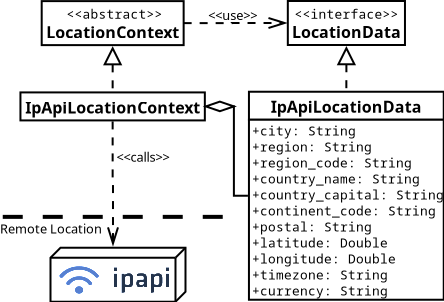
\includegraphics[width=0.76\textwidth]{img/sections/6-implementation/location-diagram-ipapi.png}
  \caption{External Service \textit{ipapi}.}
  \label{fig:impl-external-ipapi}
\end{figure}

\shorthandoff{-}